% ============================================================
%  CHAPTER 4: RELEASE 2 - WORKFLOW MANAGEMENT
% ============================================================

\fancyhead[L]{\fontsize{10}{12}\selectfont Chapter 4: Release 2 - Workflow Management}
\fancyhead[R]{}
\fancyfoot[C]{\thepage}
\pagestyle{fancy}

\phantomsection
\addcontentsline{toc}{chapter}{Chapter 4: Release 2 - Workflow Management}

% Chapter 4 follows the same figure style as Chapter 3.
\newcommand{\ChapterFourFigure}[3]{%
  \ChapterThreeFigure{#1}{#2}{#3}%
}

\newcommand{\ChapterFourFigureSized}[4]{%
  \ChapterThreeFigureSized{#1}{#2}{#3}{#4}%
}

\newcommand{\SprintThreeImplementationHeading}[1]{%
  \SprintOneImplementationHeading{#1}%
}

\newcommand{\SprintThreeScenarioHeading}[1]{%
  \SprintOneScenarioHeading{#1}%
}

\newcommand{\SprintThreeAssetPlaceholder}[2]{%
  \SprintOneAssetPlaceholder{#1}{#2}%
}

\newcommand{\SprintFourImplementationHeading}[1]{%
  \SprintThreeImplementationHeading{#1}%
}

\newcommand{\SprintFourScenarioHeading}[1]{%
  \SprintThreeScenarioHeading{#1}%
}

\newcommand{\SprintFourAssetPlaceholder}[2]{%
  \SprintThreeAssetPlaceholder{#1}{#2}%
}

\newcommand{\ChapterFourDiagramPlaceholder}[2]{%
  \SprintThreeAssetPlaceholder{#2}{#1}%
}

\begin{center}
  {\fontsize{18}{22}\selectfont \textbf{Chapter 4}}
\end{center}

\vspace{0.3cm}

\begin{center}
  {\fontsize{20}{24}\selectfont \textbf{Release 2 -- Workflow Management}}
\end{center}

\vspace{0.6cm}

% ============================================================
%  INTRODUCTION
% ============================================================
\ReportSection{Introduction}{Introduction}

{\fontsize{12}{18}\selectfont
\setlength{\parindent}{1.2cm}
\setlength{\parskip}{6pt}

\indent This chapter presents Release 2 of the ArabSoft internal platform. It focuses on workflow management through two main sprints: Sprint 3, dedicated to administrative requests, and Sprint 4, dedicated to HR management and calendar supervision. The chapter follows the same structure as the previous release by presenting the sprint goals, backlog, UML diagrams, implementation views, review, and retrospective.

}

\vspace{6pt}

% ============================================================
%  I. RELEASE ORGANIZATION
% ============================================================
\ReportSection{I. Release Organization}{I. Release Organization}

{\fontsize{12}{18}\selectfont
\setlength{\parindent}{1.2cm}
\setlength{\parskip}{6pt}

\indent Release 2 is organized around workflow management. It first covers administrative request processing through document, loan, and authorization workflows, then extends the platform with HR user supervision, organization setup, team management, and leave calendar consultation.

}

\ChapterFourFigure
{sections/chapitre4/img/other/release2_organization.png}
{Release 2 Organization}
{release2_organization}

% ============================================================
%  II. SPRINT 3: ADMINISTRATIVE REQUESTS
% ============================================================
\ReportSection{II. Sprint 3: Administrative Requests}{II. Sprint 3: Administrative Requests}

\ReportSubsection{II.1 Sprint Goal}{\hspace{0.5cm} 1. Sprint Goal}

{\fontsize{12}{18}\selectfont
\setlength{\parindent}{1.2cm}
\setlength{\parskip}{6pt}

\indent This sprint covers the administrative-request workflow of Release 2. It focuses on document requests, loan requests, authorization requests, request tracking, and the related HR decisions.

}

\ReportSubsection{II.2 Visual Sprint Journal}{\hspace{0.5cm} 2. Visual Sprint Journal}

{\fontsize{12}{18}\selectfont
\setlength{\parindent}{1.2cm}
\setlength{\parskip}{6pt}

\indent The sprint journal will capture the tracked user stories and their validation status in Jira.

}

\begin{figure}[H]
  \centering
  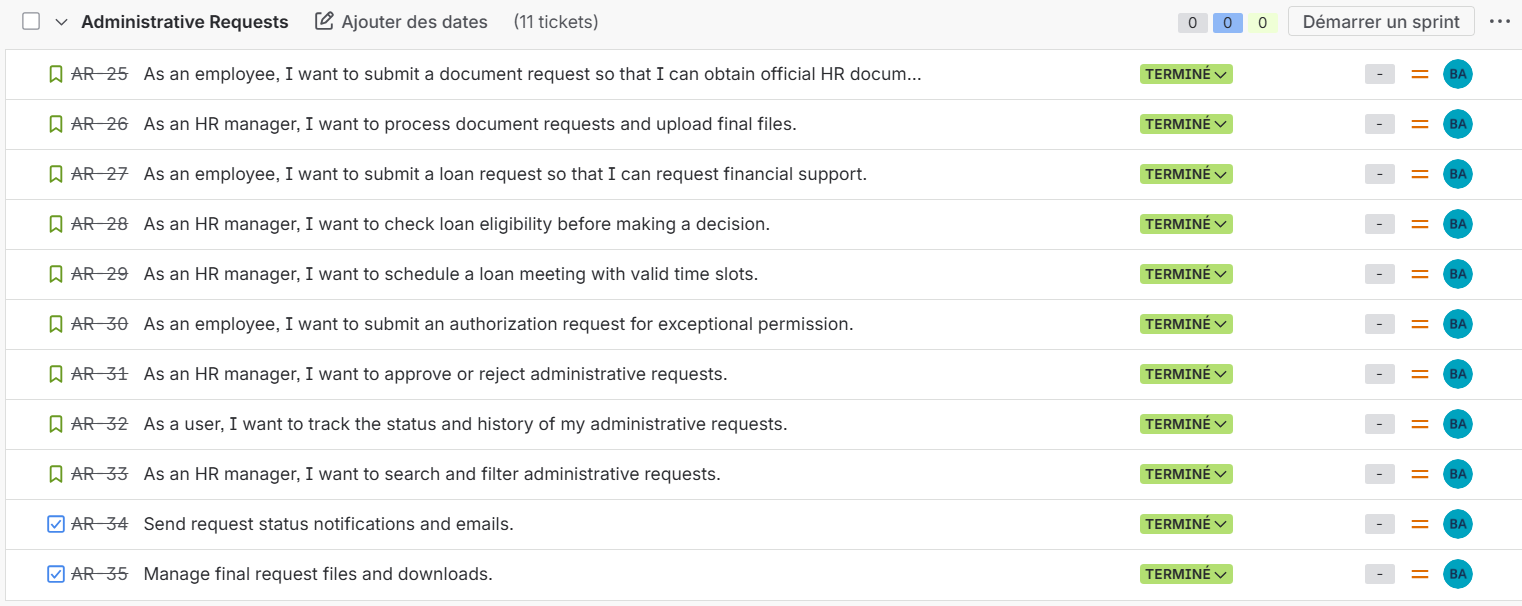
\includegraphics[width=0.95\textwidth,keepaspectratio]{sections/chapitre4/img/sprint3_administrative_requests/01_jira/sprint3_jira_journal.png}
  \caption*{Visual Sprint Journal -- Sprint 3}
  \phantomsection\label{fig:sprint3_jira_journal}
\end{figure}

\ReportSubsection{II.3 Sprint Backlog}{\hspace{0.5cm} 3. Sprint Backlog}

{\fontsize{12}{18}\selectfont
\setlength{\parindent}{1.2cm}
\setlength{\parskip}{6pt}

\indent The table below summarizes the Sprint 3 work packages prepared from the product backlog defined in Chapter 2.

}
\begin{table}[H]
\centering
\small
\renewcommand{\arraystretch}{1.36}
\setlength{\tabcolsep}{4pt}
\begin{tabular}{|>{\centering\bfseries\arraybackslash}m{1.5cm}|>{\centering\bfseries\arraybackslash}m{3.6cm}|>{\RaggedRight\arraybackslash}m{7.4cm}|>{\centering\arraybackslash}m{1.6cm}|}
\hline
\rowcolor{blue!20}
\textbf{Sprint} & \textbf{Stories} & \centering\textbf{Tasks} & \textbf{Duration} \\
\hline
\multirow{16}{=}{\centering\textbf{Sprint 3}}
& \multirow{3}{=}{\centering\textbf{Document request and processing}}
& Implement employee document request submission
& \multirow{3}{=}{\centering 2d} \\
\cline{3-3}
& & Implement HR document request processing & \\
\cline{3-3}
& & Manage final document file upload and download & \\
\cline{2-4}
& \multirow{3}{=}{\centering\textbf{Loan request and eligibility}}
& Implement employee loan request submission
& \multirow{3}{=}{\centering 2d} \\
\cline{3-3}
& & Add HR loan eligibility verification & \\
\cline{3-3}
& & Display clear loan request status and feedback & \\
\cline{2-4}
& \multirow{3}{=}{\centering\textbf{Loan meeting scheduling}}
& Implement loan meeting scheduling by HR
& \multirow{3}{=}{\centering 2d} \\
\cline{3-3}
& & Validate meeting date and available time slots & \\
\cline{3-3}
& & Prevent scheduling conflicts when applicable & \\
\cline{2-4}
& \multirow{3}{=}{\centering\textbf{Authorization request management}}
& Implement authorization request submission
& \multirow{3}{=}{\centering 2d} \\
\cline{3-3}
& & Support short absence and equipment request workflows & \\
\cline{3-3}
& & Connect HR decision handling for authorizations & \\
\cline{2-4}
& \multirow{4}{=}{\centering\textbf{Request tracking, filters, notifications, and final files}}
& Display administrative request history and status
& \multirow{4}{=}{\centering 2d} \\
\cline{3-3}
& & Add HR search and filtering for requests & \\
\cline{3-3}
& & Send request status notifications and emails & \\
\cline{3-3}
& & Manage final files for completed requests & \\
\hline
\end{tabular}
\caption{Sprint Backlog -- Sprint 3}
\label{tab:sprint3_backlog}
\end{table}

\clearpage
\ReportSubsection{II.4 Sprint Implementation}{\hspace{0.5cm} 4. Sprint Implementation}

\SprintThreeImplementationHeading{Requirements Analysis}

{\fontsize{12}{18}\selectfont
\setlength{\parindent}{1.2cm}
\setlength{\parskip}{6pt}

\indent The following analysis describes the business rules that govern each request type handled in Sprint 3, covering document requests, loan requests and meetings, authorization requests, and the HR processing and tracking logic behind each one.

}

\SprintThreeImplementationHeading{Business Rules}

{\fontsize{12}{18}\selectfont
\setlength{\parindent}{1.2cm}
\setlength{\parskip}{6pt}

\indent Employees can request official HR documents such as employment certificates, salary certificates, work reference letters, experience certificates, custom administrative letters, and leave balance statements. The leave balance statement is generated automatically after HR approval, while the other employee-requestable documents require HR to upload a final file before download. Contract copies are not submitted through the employee document request flow; they remain HR-managed through stored employee documents. Pending document requests may be approved or rejected by HR, and rejected requests require a reason.

\indent Loan requests require a type, amount, and reason. Eligibility depends on salary, seniority, and the absence of an existing active loan request. HR validation also includes meeting scheduling rules, and each decision is stored in the request history with notifications or emails.

\indent Authorization requests in the active workflow are limited to time permission and equipment request types. Time permission must respect working hours and avoid leave overlap, while equipment requests require a type, reason, and start date. HR can approve or reject each pending request with a required rejection reason.

\indent Each request is traceable through its detail view, history records, status updates, and notification events. Employee pages show personal request progress, and HR pages support search and filtering.

}

\SprintThreeImplementationHeading{Use Case Diagrams}

{\fontsize{12}{18}\selectfont
\setlength{\parindent}{1.2cm}
\setlength{\parskip}{6pt}

\indent These diagrams present the global administrative-request scope of Sprint 3 and the HR processing viewpoint for document, loan, and authorization requests.

}

\Needspace{6.2cm}
\SprintThreeScenarioHeading{Use Case Diagram -- Sprint 3 Administrative Requests}

\noindent This diagram presents the overall administrative-request scope of Sprint 3.\par

\ChapterFourFigureSized
{sections/chapitre4/img/sprint3_administrative_requests/02_use_case_diagrams/use_case_sprint3_administrative_requests.png}
{Use Case Diagram -- Sprint 3 Administrative Requests}
{use_case_sprint3_administrative_requests}
{0.92}

\Needspace{6.2cm}
\SprintThreeScenarioHeading{Use Case Diagram -- HR Administrative Request Processing}

\noindent This diagram summarizes HR processing, validation, and final decision responsibilities.\par

\ChapterFourFigureSized
{sections/chapitre4/img/sprint3_administrative_requests/02_use_case_diagrams/use_case_hr_administrative_request_processing.png}
{Use Case Diagram -- HR Administrative Request Processing}
{use_case_hr_administrative_request_processing}
{0.92}

\SprintThreeImplementationHeading{System Sequence Diagrams}

{\fontsize{12}{18}\selectfont
\setlength{\parindent}{1.2cm}
\setlength{\parskip}{6pt}

\indent These diagrams describe the main request submissions, HR processing steps, and scheduling interactions in Sprint 3.

}

\Needspace{6.2cm}
\SprintThreeScenarioHeading{System Sequence Diagram -- Submit Document Request}

\noindent This diagram shows how a user, either an employee or a team leader using employee-side request actions, submits a document request and receives validation feedback.\par

\ChapterFourFigureSized
{sections/chapitre4/img/sprint3_administrative_requests/03_system_sequence_diagrams/ssd_submit_document_request.png}
{System Sequence Diagram -- Submit Document Request}
{ssd_submit_document_request}
{0.92}

\Needspace{6.2cm}
\SprintThreeScenarioHeading{System Sequence Diagram -- Process Document Request}

\noindent This diagram shows how HR processes a pending document request and manages the final file.\par

\ChapterFourFigureSized
{sections/chapitre4/img/sprint3_administrative_requests/03_system_sequence_diagrams/ssd_process_document_request.png}
{System Sequence Diagram -- Process Document Request}
{ssd_process_document_request}
{0.92}

\Needspace{6.2cm}
\SprintThreeScenarioHeading{System Sequence Diagram -- Submit Loan Request}

\noindent This diagram shows how a user, either an employee or a team leader using employee-side request actions, submits a loan request with the required request data.\par

\ChapterFourFigureSized
{sections/chapitre4/img/sprint3_administrative_requests/03_system_sequence_diagrams/ssd_submit_loan_request.png}
{System Sequence Diagram -- Submit Loan Request}
{ssd_submit_loan_request}
{0.92}

\Needspace{6.2cm}
\SprintThreeScenarioHeading{System Sequence Diagram -- Schedule Loan Meeting}

\noindent This diagram shows how HR schedules a loan meeting under the workflow constraints.\par

\ChapterFourFigureSized
{sections/chapitre4/img/sprint3_administrative_requests/03_system_sequence_diagrams/ssd_schedule_loan_meeting.png}
{System Sequence Diagram -- Schedule Loan Meeting}
{ssd_schedule_loan_meeting}
{0.92}

\Needspace{6.2cm}
\SprintThreeScenarioHeading{System Sequence Diagram -- Submit Authorization Request}

\noindent This diagram shows how a user, either an employee or a team leader using employee-side request actions, submits a time permission or equipment request.\par

\ChapterFourFigureSized
{sections/chapitre4/img/sprint3_administrative_requests/03_system_sequence_diagrams/ssd_submit_authorization_request.png}
{System Sequence Diagram -- Submit Authorization Request}
{ssd_submit_authorization_request}
{0.92}

\Needspace{6.2cm}
\SprintThreeScenarioHeading{System Sequence Diagram -- HR Administrative Request Decision}

\noindent This diagram shows how HR approves or rejects a pending administrative request.\par

\ChapterFourFigureSized
{sections/chapitre4/img/sprint3_administrative_requests/03_system_sequence_diagrams/ssd_hr_administrative_request_decision.png}
{System Sequence Diagram -- HR Administrative Request Decision}
{ssd_hr_administrative_request_decision}
{0.92}

\SprintThreeImplementationHeading{Analysis}

{\fontsize{12}{18}\selectfont
\setlength{\parindent}{1.2cm}
\setlength{\parskip}{6pt}

\indent The analysis covers the main domain concepts in Sprint 3: the request entities, decision traces, and final-file handling across the three request types.

}

\Needspace{6.2cm}

\SprintThreeScenarioHeading{Domain Model -- Sprint 3 Administrative Requests}

\noindent This diagram presents the main domain concepts used to manage Sprint 3 administrative requests, including document requests, loan requests, authorization requests, request history, stored employee documents, and the related status and type values.\par

\ChapterFourFigureSized
{sections/chapitre4/img/sprint3_administrative_requests/05_domain_model/domain_model_sprint3_administrative_requests.png}
{Domain Model -- Sprint 3 Administrative Requests}
{domain_model_sprint3_administrative_requests}
{0.92}
\SprintThreeImplementationHeading{Participant Class Diagrams}

{\fontsize{12}{18}\selectfont
\setlength{\parindent}{1.2cm}
\setlength{\parskip}{6pt}

\indent These diagrams identify the main frontend and backend participants involved in employee administrative request submission and HR request processing during Sprint 3.

}

\Needspace{7.2cm}
\SprintThreeScenarioHeading{Participant Class Diagram -- Document Request Management}

\noindent This diagram shows the participants involved in employee document request submission, draft validation, status tracking, and request history management.\par

\ChapterFourFigureSized
{sections/chapitre4/img/sprint3_administrative_requests/06_participant_class_diagrams/participant_document_request_management.png}
{Participant Class Diagram -- Document Request Management}
{participant_document_request_management}
{0.95}

\Needspace{7.2cm}
\SprintThreeScenarioHeading{Participant Class Diagram -- Loan Request Management}

\noindent This diagram shows the participants involved in employee loan request submission, draft validation, eligibility evaluation, status tracking, and request history management.\par

\ChapterFourFigureSized
{sections/chapitre4/img/sprint3_administrative_requests/06_participant_class_diagrams/participant_loan_request_management.png}
{Participant Class Diagram -- Loan Request Management}
{participant_loan_request_management}
{0.95}

\Needspace{7.2cm}
\SprintThreeScenarioHeading{Participant Class Diagram -- Authorization Request Management}

\noindent This diagram shows the participants involved in employee authorization request submission, draft validation, status tracking, and request history management.\par

\ChapterFourFigureSized
{sections/chapitre4/img/sprint3_administrative_requests/06_participant_class_diagrams/participant_authorization_request_management.png}
{Participant Class Diagram -- Authorization Request Management}
{participant_authorization_request_management}
{0.95}

\Needspace{7.2cm}
\SprintThreeScenarioHeading{Participant Class Diagram -- HR Request Processing}

\noindent This diagram shows the participants involved in HR processing of document, loan, and authorization requests, including request review, status updates, and history tracking.\par

\ChapterFourFigureSized
{sections/chapitre4/img/sprint3_administrative_requests/06_participant_class_diagrams/participant_hr_request_processing.png}
{Participant Class Diagram -- HR Request Processing}
{participant_hr_request_processing}
{0.95}
\SprintThreeImplementationHeading{State Diagrams}

{\fontsize{12}{18}\selectfont
\setlength{\parindent}{1.2cm}
\setlength{\parskip}{6pt}

\indent These diagrams summarize the lifecycle states and transitions used by document, loan, and authorization requests during Sprint 3. They distinguish real backend request statuses from derived display outcomes such as document readiness or waiting for an HR-uploaded file.

}

\Needspace{6.2cm}
\SprintThreeScenarioHeading{State Diagram -- Document Request Lifecycle}

\noindent This diagram shows the lifecycle of a document request from submission to HR decision, including the derived fulfillment outcomes used when a leave balance statement is immediately ready or another document is waiting for an HR-uploaded file.\par

\ChapterFourFigureSized
{sections/chapitre4/img/sprint3_administrative_requests/04_state_diagrams/state_document_request_lifecycle.png}
{State Diagram -- Document Request Lifecycle}
{state_document_request_lifecycle}
{0.90}

\Needspace{6.2cm}
\SprintThreeScenarioHeading{State Diagram -- Loan Request Lifecycle}

\noindent This diagram shows the lifecycle of a loan request, including meeting and final decision states.\par

\ChapterFourFigureSized
{sections/chapitre4/img/sprint3_administrative_requests/04_state_diagrams/state_loan_request_lifecycle.png}
{State Diagram -- Loan Request Lifecycle}
{state_loan_request_lifecycle}
{0.90}

\Needspace{6.2cm}
\SprintThreeScenarioHeading{State Diagram -- Authorization Request Lifecycle}

\noindent This diagram shows the lifecycle of an authorization request from submission to HR decision.\par

\ChapterFourFigureSized
{sections/chapitre4/img/sprint3_administrative_requests/04_state_diagrams/state_authorization_request_lifecycle.png}
{State Diagram -- Authorization Request Lifecycle}
{state_authorization_request_lifecycle}
{0.90}

\SprintThreeImplementationHeading{Design Class Diagrams}

{\fontsize{12}{18}\selectfont
\setlength{\parindent}{1.2cm}
\setlength{\parskip}{6pt}

\indent These diagrams present the main design classes that support document handling, loan eligibility, authorization decisions, and history tracking.

}

\Needspace{6.2cm}
\SprintThreeScenarioHeading{Design Class Diagram -- Document Request Final File Management}

\noindent This diagram shows the classes used to manage generated documents and HR-uploaded final files.\par

\ChapterFourFigureSized
{sections/chapitre4/img/sprint3_administrative_requests/07_design_class_diagrams/design_document_request_final_file_management.png}
{Design Class Diagram -- Document Request Final File Management}
{design_document_request_final_file_management}
{0.95}

\Needspace{6.2cm}
\SprintThreeScenarioHeading{Design Class Diagram -- Loan Eligibility and Meeting Management}

\noindent This diagram shows the classes used to verify loan eligibility and manage loan meetings.\par

\ChapterFourFigureSized
{sections/chapitre4/img/sprint3_administrative_requests/07_design_class_diagrams/design_loan_request_review_management.png}
{Design Class Diagram -- Loan Request Review Management}
{design_loan_request_review_management}
{0.95}

\Needspace{6.2cm}
\SprintThreeScenarioHeading{Design Class Diagram -- Authorization Request Decision Management}

\noindent This diagram shows the classes used to process authorization decisions and rejection reasons.\par

\ChapterFourFigureSized
{sections/chapitre4/img/sprint3_administrative_requests/07_design_class_diagrams/design_authorization_request_management.png}
{Design Class Diagram -- Authorization Request Management}
{design_authorization_request_management}
{0.95}

\Needspace{6.2cm}
\SprintThreeScenarioHeading{Design Class Diagram -- Request History and Notification Management}

\noindent This diagram shows the classes used to trace history and emit request events and notifications.\par

\ChapterFourFigureSized
{sections/chapitre4/img/sprint3_administrative_requests/07_design_class_diagrams/design_hr_request_processing.png}
{Design Class Diagram -- HR Request Processing}
{design_hr_request_processing}
{0.95}

\SprintThreeImplementationHeading{Conception Sequence Diagrams}

{\fontsize{12}{18}\selectfont
\setlength{\parindent}{1.2cm}
\setlength{\parskip}{6pt}

\indent These diagrams describe the internal frontend and backend interactions behind the administrative request workflows of Sprint 3. They are organized by request category: document requests, loan requests, and authorization requests. Each workflow is split into focused frontend and backend views to keep the diagrams readable and to separate user-interface behavior from backend validation, persistence, history, and notification logic.

}

\Needspace{6.2cm}
\SprintThreeScenarioHeading{Conception Sequence Diagram -- Document Request HR Decision Frontend}

\ChapterFourFigureSized
{sections/chapitre4/img/sprint3_administrative_requests/08_conception_sequence_diagrams/csd_document_request_hr_decision_frontend.png}
{Conception Sequence Diagram -- Document Request HR Decision Frontend}
{sprint3_csd_document_request_hr_decision_frontend}
{0.95}

\Needspace{6.2cm}
\SprintThreeScenarioHeading{Conception Sequence Diagram -- Document Request Decision Backend}

\ChapterFourFigureSized
{sections/chapitre4/img/sprint3_administrative_requests/08_conception_sequence_diagrams/csd_document_request_decision_backend.png}
{Conception Sequence Diagram -- Document Request Decision Backend}
{sprint3_csd_document_request_decision_backend}
{0.95}

\Needspace{6.2cm}
\SprintThreeScenarioHeading{Conception Sequence Diagram -- Document Request Final File Frontend}

\ChapterFourFigureSized
{sections/chapitre4/img/sprint3_administrative_requests/08_conception_sequence_diagrams/csd_document_request_final_file_frontend.png}
{Conception Sequence Diagram -- Document Request Final File Frontend}
{sprint3_csd_document_request_final_file_frontend}
{0.95}

\Needspace{6.2cm}
\SprintThreeScenarioHeading{Conception Sequence Diagram -- Document Request Final File Backend}

\ChapterFourFigureSized
{sections/chapitre4/img/sprint3_administrative_requests/08_conception_sequence_diagrams/csd_document_request_final_file_backend.png}
{Conception Sequence Diagram -- Document Request Final File Backend}
{sprint3_csd_document_request_final_file_backend}
{0.98}

\Needspace{6.2cm}
\SprintThreeScenarioHeading{Conception Sequence Diagram -- Loan Request Submission Frontend}

\ChapterFourFigureSized
{sections/chapitre4/img/sprint3_administrative_requests/08_conception_sequence_diagrams/csd_loan_request_submission_frontend.png}
{Conception Sequence Diagram -- Loan Request Submission Frontend}
{sprint3_csd_loan_request_submission_frontend}
{0.95}

\Needspace{6.2cm}
\SprintThreeScenarioHeading{Conception Sequence Diagram -- Loan Request Submission Backend}

\ChapterFourFigureSized
{sections/chapitre4/img/sprint3_administrative_requests/08_conception_sequence_diagrams/csd_loan_request_submission_backend.png}
{Conception Sequence Diagram -- Loan Request Submission Backend}
{sprint3_csd_loan_request_submission_backend}
{0.98}

\Needspace{6.2cm}
\SprintThreeScenarioHeading{Conception Sequence Diagram -- Loan Request Meeting Scheduling Frontend}

\ChapterFourFigureSized
{sections/chapitre4/img/sprint3_administrative_requests/08_conception_sequence_diagrams/csd_loan_request_meeting_frontend.png}
{Conception Sequence Diagram -- Loan Request Meeting Scheduling Frontend}
{sprint3_csd_loan_request_meeting_frontend}
{0.95}

\Needspace{6.2cm}
\SprintThreeScenarioHeading{Conception Sequence Diagram -- Loan Meeting Scheduling Backend}

\ChapterFourFigureSized
{sections/chapitre4/img/sprint3_administrative_requests/08_conception_sequence_diagrams/csd_loan_request_meeting_backend.png}
{Conception Sequence Diagram -- Loan Meeting Scheduling Backend}
{sprint3_csd_loan_request_meeting_backend}
{0.95}

\Needspace{6.2cm}
\SprintThreeScenarioHeading{Conception Sequence Diagram -- Loan Request Decision Frontend}

\ChapterFourFigureSized
{sections/chapitre4/img/sprint3_administrative_requests/08_conception_sequence_diagrams/csd_loan_request_decision_frontend.png}
{Conception Sequence Diagram -- Loan Request Decision Frontend}
{sprint3_csd_loan_request_decision_frontend}
{0.95}

\Needspace{6.2cm}
\SprintThreeScenarioHeading{Conception Sequence Diagram -- Loan Request Decision Backend}

\ChapterFourFigureSized
{sections/chapitre4/img/sprint3_administrative_requests/08_conception_sequence_diagrams/csd_loan_request_decision_backend.png}
{Conception Sequence Diagram -- Loan Request Decision Backend}
{sprint3_csd_loan_request_decision_backend}
{0.98}

\Needspace{6.2cm}
\SprintThreeScenarioHeading{Conception Sequence Diagram -- Loan Final File Delivery Frontend}

\ChapterFourFigureSized
{sections/chapitre4/img/sprint3_administrative_requests/08_conception_sequence_diagrams/csd_loan_request_final_file_frontend.png}
{Conception Sequence Diagram -- Loan Final File Delivery Frontend}
{sprint3_csd_loan_request_final_file_frontend}
{0.95}

\Needspace{6.2cm}
\SprintThreeScenarioHeading{Conception Sequence Diagram -- Loan Final File Backend}

\ChapterFourFigureSized
{sections/chapitre4/img/sprint3_administrative_requests/08_conception_sequence_diagrams/csd_loan_request_final_file_backend.png}
{Conception Sequence Diagram -- Loan Final File Backend}
{sprint3_csd_loan_request_final_file_backend}
{0.95}

\Needspace{6.2cm}
\SprintThreeScenarioHeading{Conception Sequence Diagram -- Authorization Request Submission Frontend}

\ChapterFourFigureSized
{sections/chapitre4/img/sprint3_administrative_requests/08_conception_sequence_diagrams/csd_authorization_request_submission_frontend.png}
{Conception Sequence Diagram -- Authorization Request Submission Frontend}
{sprint3_csd_authorization_request_submission_frontend}
{0.95}

\Needspace{6.2cm}
\SprintThreeScenarioHeading{Conception Sequence Diagram -- Authorization Request Submission Backend}

\ChapterFourFigureSized
{sections/chapitre4/img/sprint3_administrative_requests/08_conception_sequence_diagrams/csd_authorization_request_submission_backend.png}
{Conception Sequence Diagram -- Authorization Request Submission Backend}
{sprint3_csd_authorization_request_submission_backend}
{0.98}

\Needspace{6.2cm}
\SprintThreeScenarioHeading{Conception Sequence Diagram -- Authorization Request Decision Frontend}

\ChapterFourFigureSized
{sections/chapitre4/img/sprint3_administrative_requests/08_conception_sequence_diagrams/csd_authorization_request_decision_frontend.png}
{Conception Sequence Diagram -- Authorization Request Decision Frontend}
{sprint3_csd_authorization_request_decision_frontend}
{0.95}

\Needspace{6.2cm}
\SprintThreeScenarioHeading{Conception Sequence Diagram -- Authorization Request Decision Backend}

\ChapterFourFigureSized
{sections/chapitre4/img/sprint3_administrative_requests/08_conception_sequence_diagrams/csd_authorization_request_decision_backend.png}
{Conception Sequence Diagram -- Authorization Request Decision Backend}
{sprint3_csd_authorization_request_decision_backend}
{0.98}

\SprintThreeImplementationHeading{Realization}

{\fontsize{12}{18}\selectfont
\setlength{\parindent}{1.2cm}
\setlength{\parskip}{6pt}

\indent The realization section presents the validated user interfaces for Sprint 3.

}

\Needspace{7.2cm}
\begin{figure}[H]
  \centering
  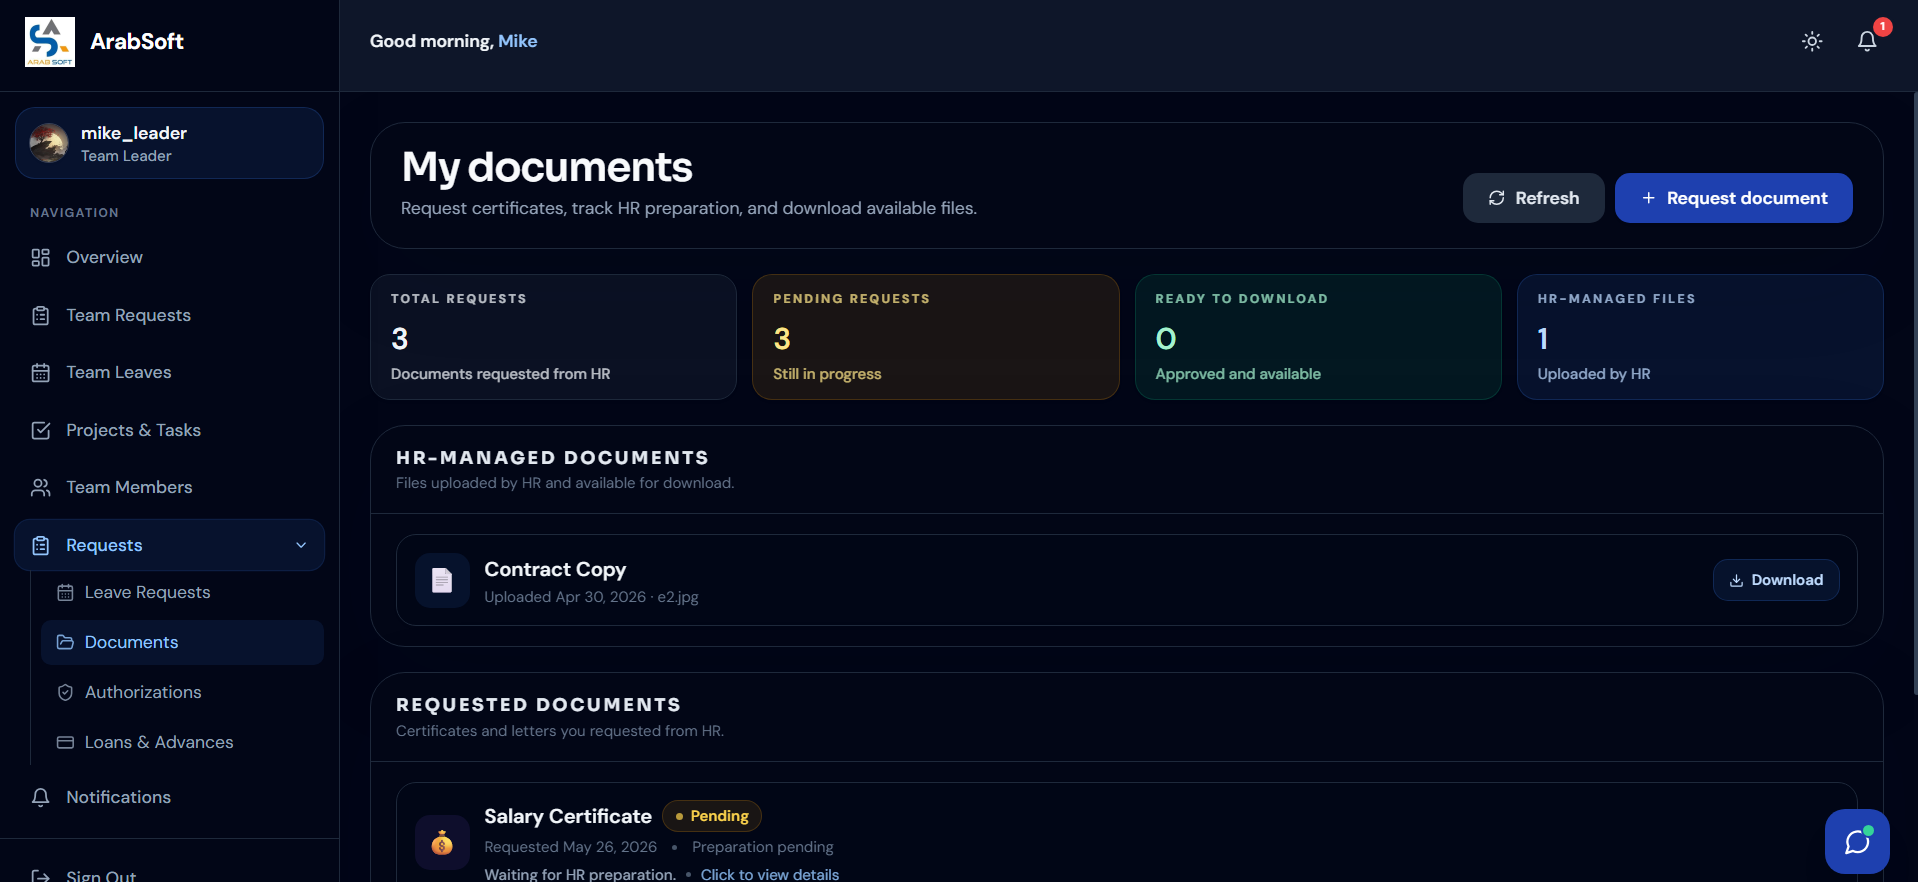
\includegraphics[width=0.95\textwidth,keepaspectratio]{sections/chapitre4/img/sprint3_administrative_requests/09_ui_screenshots/ui_employee_documents_page.png}
  \caption{Employee Documents Interface}
  \label{fig:sprint3_employee_documents_ui}
\end{figure}

\Needspace{7.2cm}
\begin{figure}[H]
  \centering
  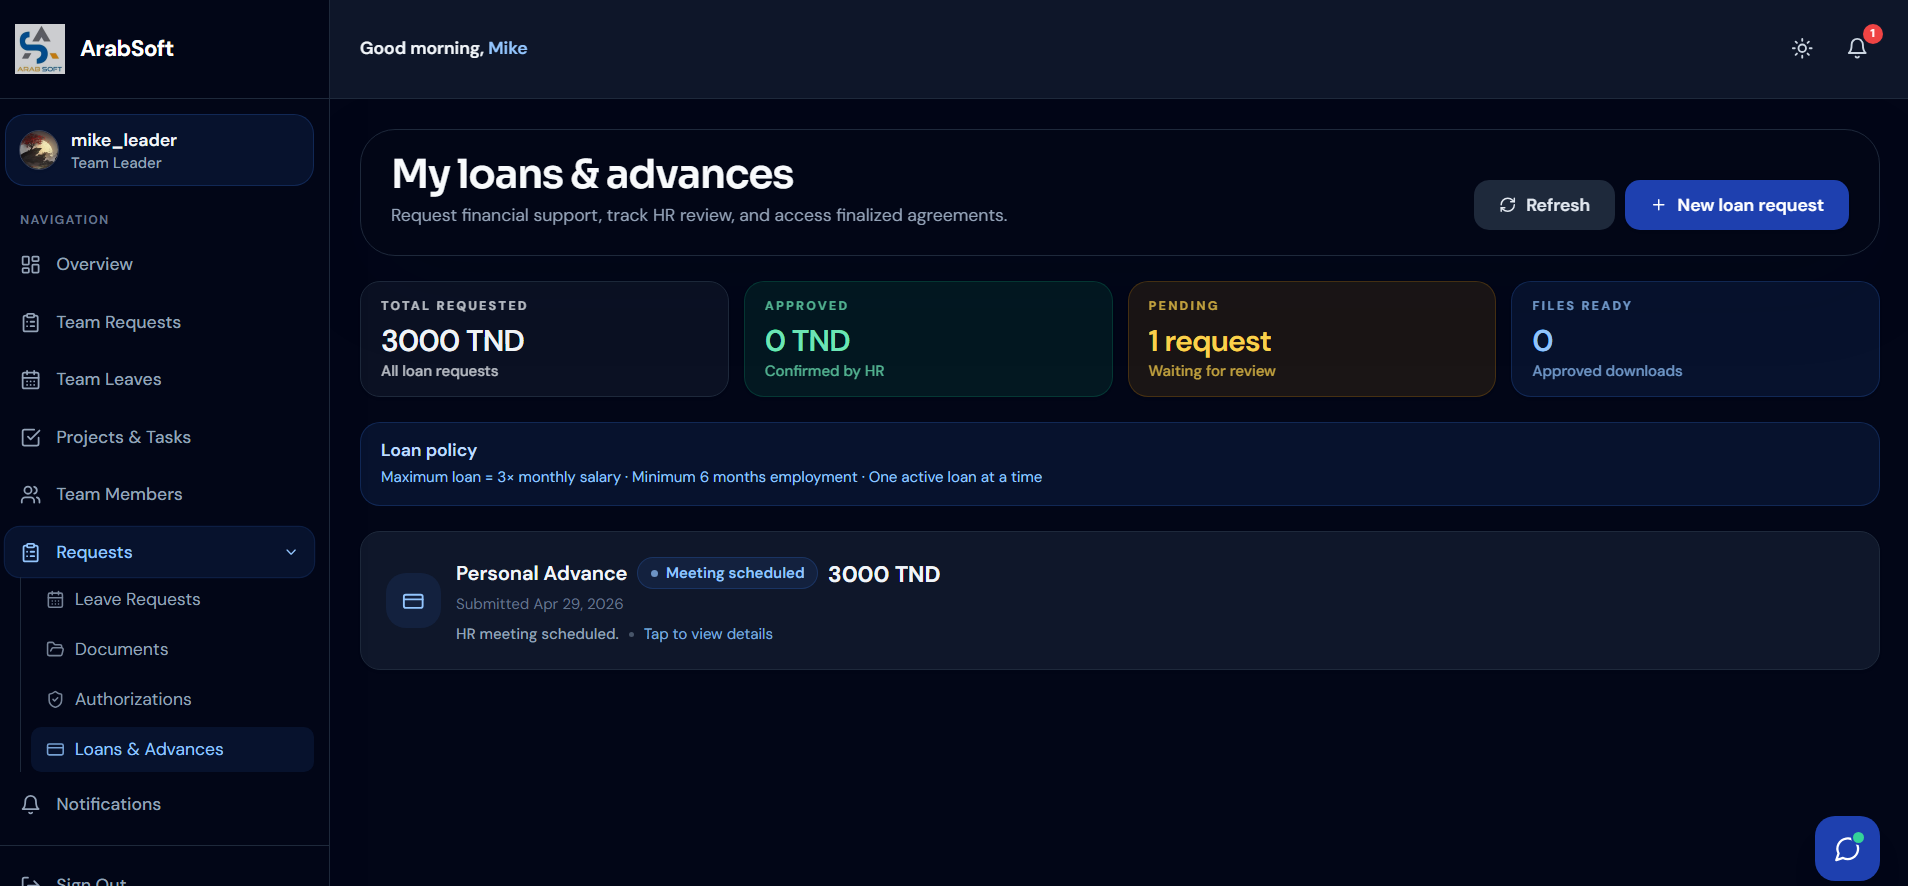
\includegraphics[width=0.95\textwidth,keepaspectratio]{sections/chapitre4/img/sprint3_administrative_requests/09_ui_screenshots/ui_employee_loans_page.png}
  \caption{Employee Loans and Advances Interface}
  \label{fig:sprint3_employee_loans_ui}
\end{figure}

\Needspace{7.2cm}
\begin{figure}[H]
  \centering
  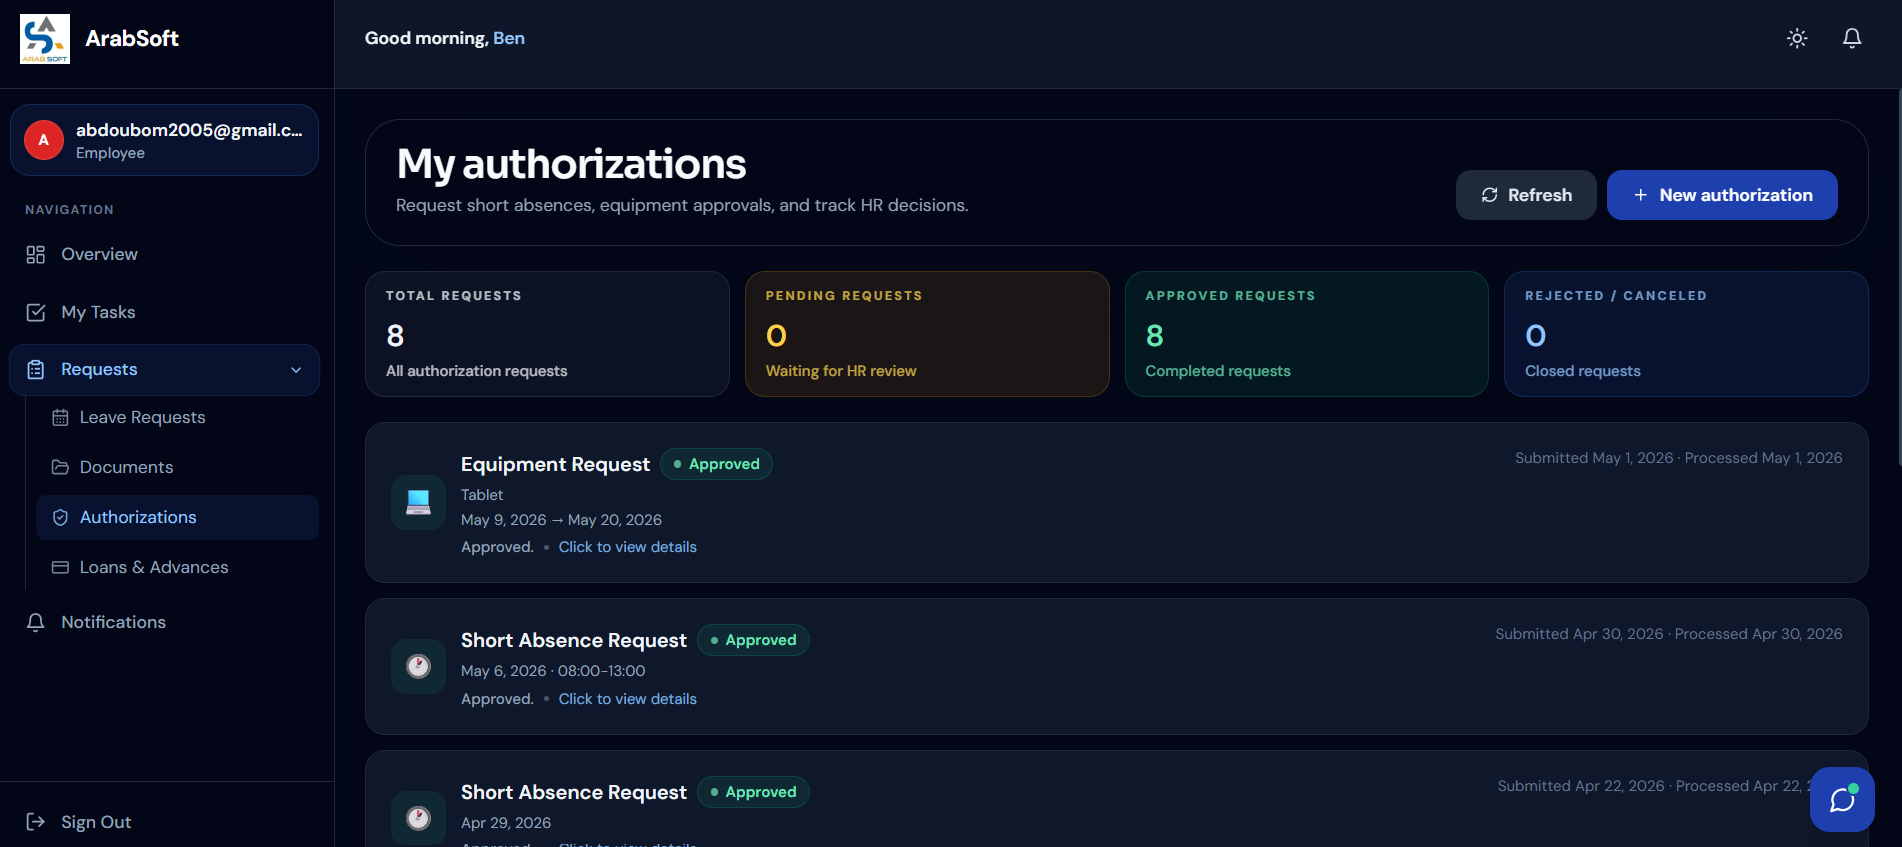
\includegraphics[width=0.95\textwidth,keepaspectratio]{sections/chapitre4/img/sprint3_administrative_requests/09_ui_screenshots/ui_employee_authorizations_page.png}
  \caption{Employee Authorizations Interface}
  \label{fig:sprint3_employee_authorizations_ui}
\end{figure}

\Needspace{7.2cm}
\begin{figure}[H]
  \centering
  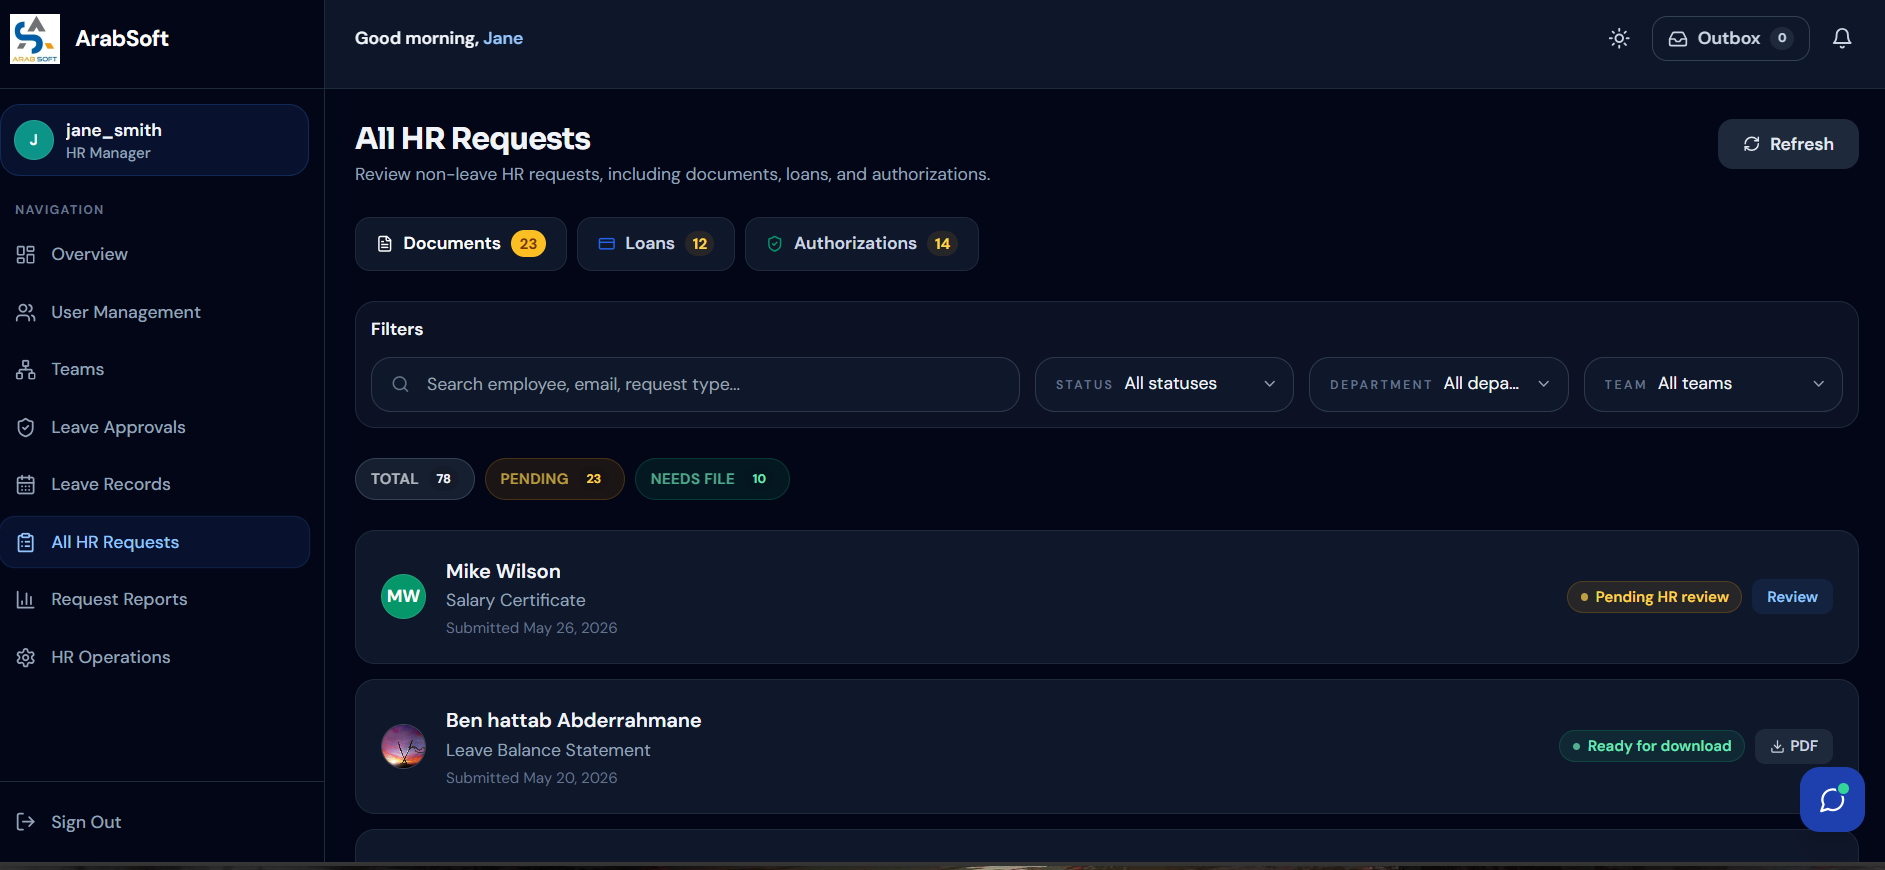
\includegraphics[width=0.95\textwidth,keepaspectratio]{sections/chapitre4/img/sprint3_administrative_requests/09_ui_screenshots/ui_hr_requests_page.png}
  \caption{HR Administrative Requests Interface}
  \label{fig:sprint3_hr_requests_ui}
\end{figure}

\Needspace{7.2cm}
\begin{figure}[H]
  \centering
  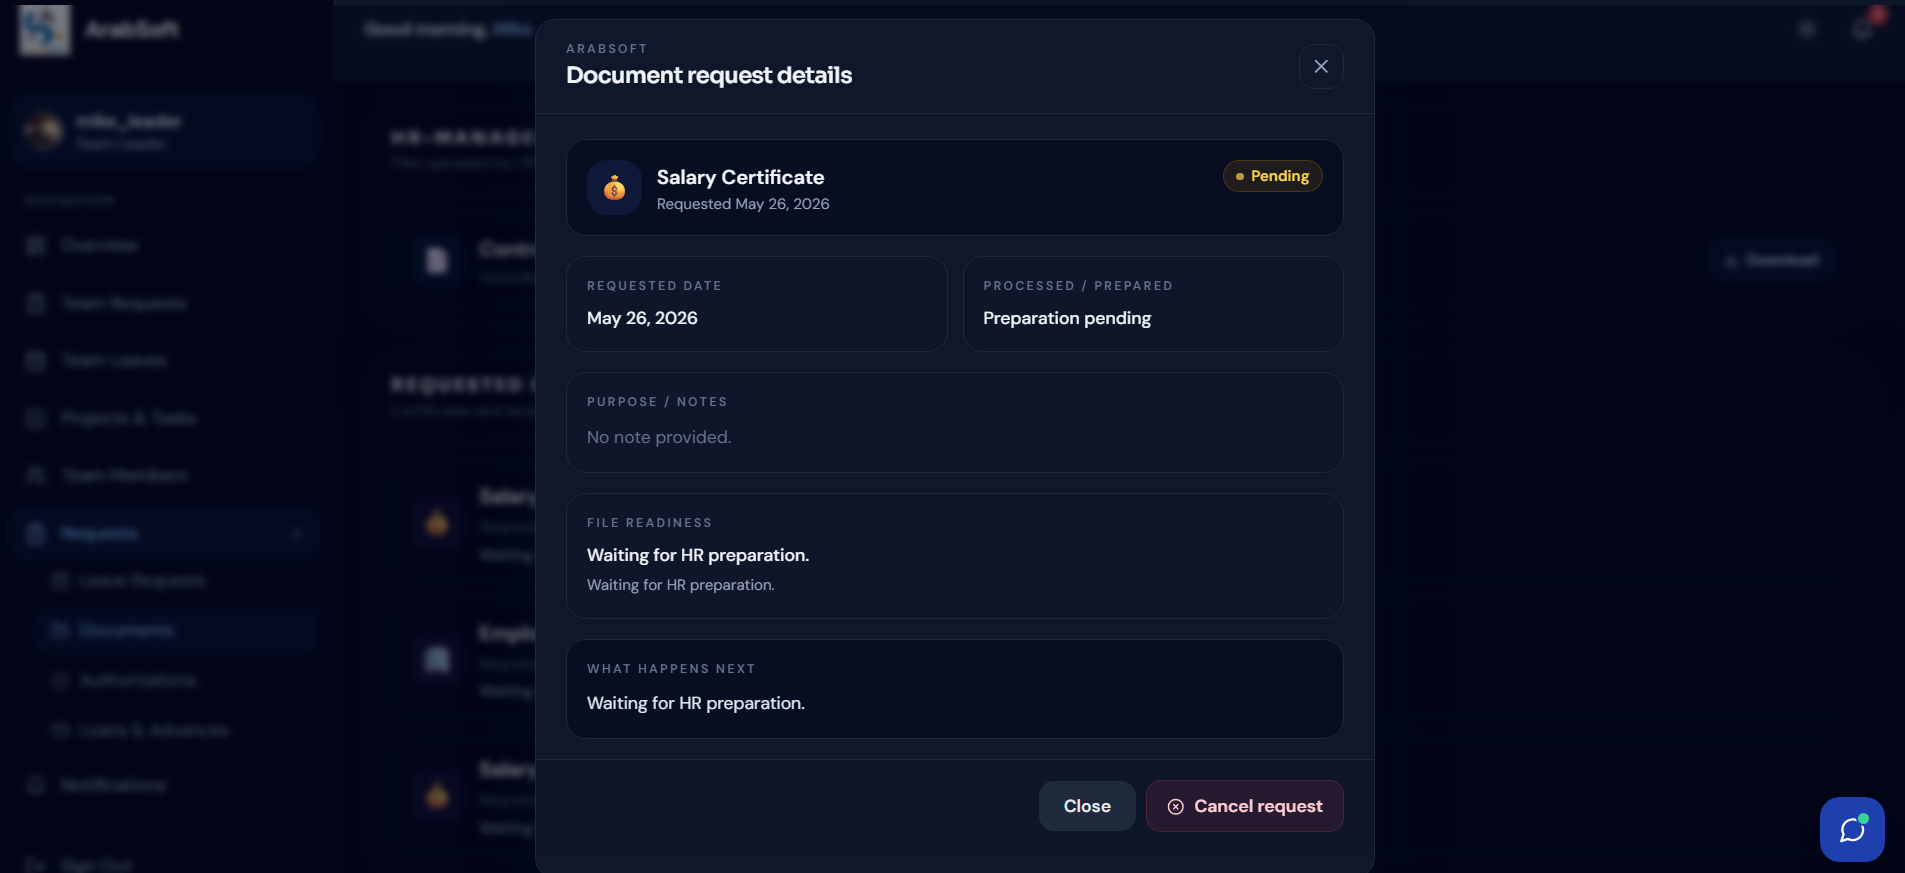
\includegraphics[width=0.95\textwidth,keepaspectratio]{sections/chapitre4/img/sprint3_administrative_requests/09_ui_screenshots/ui_request_detail_history.png}
  \caption{Request Detail and History Interface}
  \label{fig:sprint3_request_detail_history_ui}
\end{figure}

\ReportSubsection{II.5 Sprint Review}{\hspace{0.5cm} 5. Sprint Review}

{\fontsize{12}{18}\selectfont
\setlength{\parindent}{1.2cm}
\setlength{\parskip}{6pt}

\indent Sprint 3 covered the administrative request workflow of the platform. Employees can submit and track document, loan, and authorization requests. HR managers can review each request, approve or reject it with a decision note, schedule loan meetings, upload final files where required, and consult the full request history. Request statuses, history records, decision notes, and notification events keep each request traceable from submission through to final decision. Final-file handling for document and loan requests was also built into the workflow.

}

\ReportSubsection{II.6 Sprint Retrospective}{\hspace{0.5cm} 6. Sprint Retrospective}

\begin{table}[H]
\centering
\renewcommand{\arraystretch}{1.5}
\setlength{\tabcolsep}{6pt}
\begin{tabular}{|>{\centering\bfseries\arraybackslash}m{5.2cm}|>{\centering\bfseries\arraybackslash}m{5.2cm}|}
\hline
\rowcolor{blue!20}
\textbf{What went well} & \textbf{What needs improvement} \\
\hline
The sprint delivered the main administrative request workflows for documents, loans, and authorizations.
&
Workflow complexity required tighter validation rules and a clearer HR decision flow across request states.
\\
\hline
Request history, decision notes, statuses, and notifications improved workflow traceability.
&
Final-file handling and edge-case paths still need clearer validation and traceability.
\\
\hline
Splitting frontend and backend diagrams made the technical design easier to explain.
&
UI validation and user testing still need to cover feedback messages and request-state transitions.
\\
\hline
\end{tabular}
\caption{Sprint Retrospective -- Sprint 3}
\label{tab:sprint3_retrospective}
\end{table}

\clearpage
% ============================================================
%  III. SPRINT 4: HR MANAGEMENT AND CALENDAR
% ============================================================
\ReportSection{III. Sprint 4: HR Management and Calendar}{III. Sprint 4: HR Management and Calendar}

\ReportSubsection{III.1 Sprint Goal}{\hspace{0.5cm} 1. Sprint Goal}

{\fontsize{12}{18}\selectfont
\setlength{\parindent}{1.2cm}
\setlength{\parskip}{6pt}

\indent This sprint covers HR management and calendar supervision. It handles HR user administration, employee records, team setup, role assignment, account activation and deactivation, and leave-availability views for employees and teams.

}

\ReportSubsection{III.2 Visual Sprint Journal}{\hspace{0.5cm} 2. Visual Sprint Journal}

{\fontsize{12}{18}\selectfont
\setlength{\parindent}{1.2cm}
\setlength{\parskip}{6pt}

\indent The sprint journal captures the tracked HR and calendar user stories and their validation status in Jira.

}

\begin{figure}[H]
  \centering
  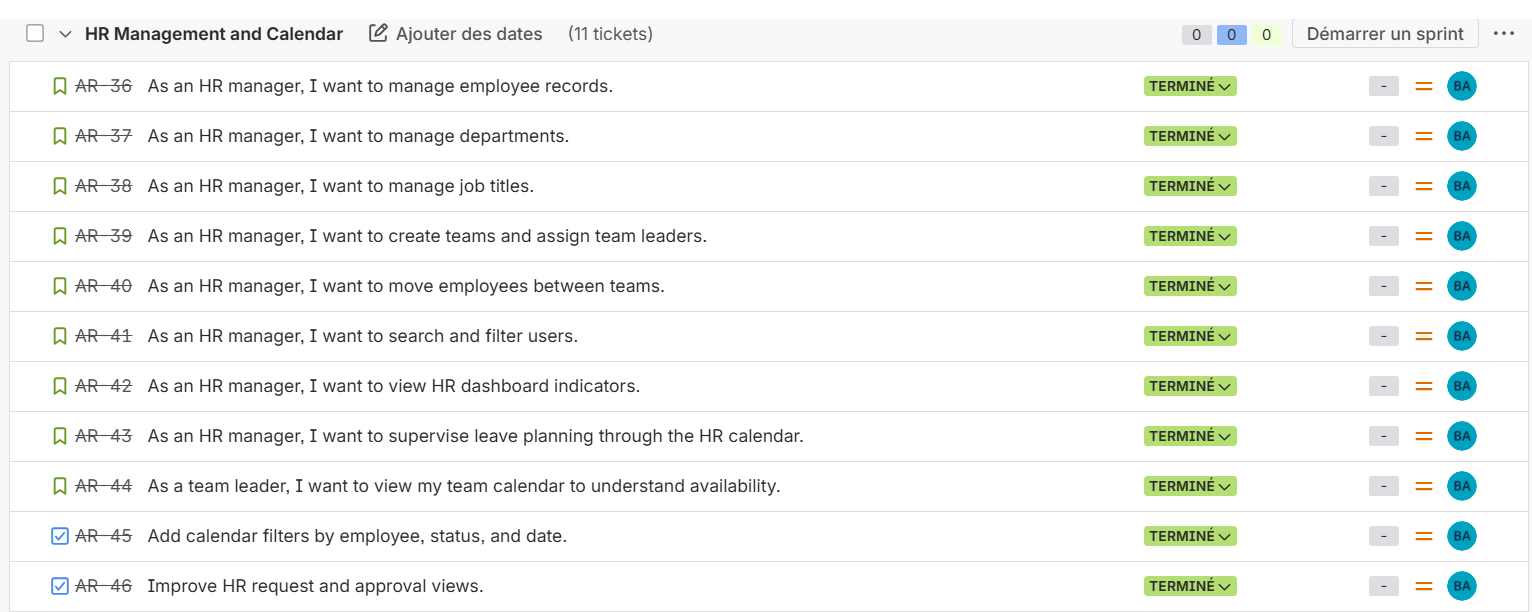
\includegraphics[width=0.95\textwidth,keepaspectratio]{sections/chapitre4/img/sprint4_hr_management_calendar/01_jira/sprint4_jira_journal.png}
  \caption*{Visual Sprint Journal -- Sprint 4}
  \phantomsection\label{fig:sprint4_jira_journal}
\end{figure}

\ReportSubsection{III.3 Sprint Backlog}{\hspace{0.5cm} 3. Sprint Backlog}

{\fontsize{12}{18}\selectfont
\setlength{\parindent}{1.2cm}
\setlength{\parskip}{6pt}

\indent The table below summarizes the Sprint 4 work packages prepared from the product backlog defined in Chapter 2.

}

% TODO: insert the Sprint 4 backlog table after validating the relevant Chapter 2 backlog items.
\begin{table}[H]
\centering
\small
\renewcommand{\arraystretch}{1.36}
\setlength{\tabcolsep}{4pt}
\begin{tabular}{|>{\centering\bfseries\arraybackslash}m{1.5cm}|>{\centering\bfseries\arraybackslash}m{3.6cm}|>{\RaggedRight\arraybackslash}m{7.4cm}|>{\centering\arraybackslash}m{1.6cm}|}
\hline
\rowcolor{blue!20}
\textbf{Sprint} & \textbf{Stories} & \centering\textbf{Tasks} & \textbf{Duration} \\
\hline
\multirow{18}{=}{\centering\textbf{Sprint 4}}
& \multirow{3}{=}{\centering\textbf{Employee records and user search}}
& Implement employee record consultation and update
& \multirow{3}{=}{\centering 2d} \\
\cline{3-3}
& & Add user search and filtering for HR & \\
\cline{3-3}
& & Improve employee profile visibility for HR & \\
\cline{2-4}
& \multirow{3}{=}{\centering\textbf{Department and job title management}}
& Implement department management
& \multirow{3}{=}{\centering 2d} \\
\cline{3-3}
& & Implement job title management & \\
\cline{3-3}
& & Connect departments and job titles with employee records & \\
\cline{2-4}
& \multirow{3}{=}{\centering\textbf{Team management and leader assignment}}
& Implement team creation and update
& \multirow{3}{=}{\centering 2d} \\
\cline{3-3}
& & Assign or change team leaders & \\
\cline{3-3}
& & Handle teams without assigned leaders when needed & \\
\cline{2-4}
& \multirow{3}{=}{\centering\textbf{Employee movement and HR approval views}}
& Move employees between teams
& \multirow{3}{=}{\centering 1d} \\
\cline{3-3}
& & Improve HR request and approval views & \\
\cline{3-3}
& & Keep employee assignment data consistent & \\
\cline{2-4}
& \multirow{3}{=}{\centering\textbf{HR dashboard and HR calendar}}
& Display HR dashboard indicators
& \multirow{3}{=}{\centering 2d} \\
\cline{3-3}
& & Implement HR leave calendar supervision & \\
\cline{3-3}
& & Add calendar visibility for employees, teams, and statuses & \\
\cline{2-4}
& \multirow{3}{=}{\centering\textbf{Team calendar and calendar filters}}
& Implement team calendar consultation
& \multirow{3}{=}{\centering 1d} \\
\cline{3-3}
& & Add calendar filters by employee, status, and date & \\
\cline{3-3}
& & Improve calendar readability for planning & \\
\hline
\end{tabular}
\caption{Sprint Backlog -- Sprint 4}
\label{tab:sprint4_backlog}
\end{table}

\clearpage
\ReportSubsection{III.4 Sprint Implementation}{\hspace{0.5cm} 4. Sprint Implementation}

\SprintFourImplementationHeading{Requirements Analysis}

{\fontsize{12}{18}\selectfont
\setlength{\parindent}{1.2cm}
\setlength{\parskip}{6pt}

\indent Sprint 4 covers HR management and calendar supervision, including the HR dashboard, employee account supervision, organization setup, team structure management, and leave calendar views.

}

\ChapterFourFigureSized
{sections/chapitre4/img/sprint4_hr_management_calendar/02_use_case_diagrams/use_case_sprint4_hr_management_calendar.png}
{Use Case Diagram -- Sprint 4 HR Management and Calendar}
{use_case_sprint4_hr_management_calendar}
{0.92}

\ChapterFourFigureSized
{sections/chapitre4/img/sprint4_hr_management_calendar/02_use_case_diagrams/use_case_sprint4_hr_employee_account_supervision.png}
{Use Case Diagram -- HR Employee and Account Supervision}
{use_case_sprint4_hr_employee_account_supervision}
{0.92}

\ChapterFourFigureSized
{sections/chapitre4/img/sprint4_hr_management_calendar/02_use_case_diagrams/use_case_sprint4_organization_team_management.png}
{Use Case Diagram -- Organization and Team Management}
{use_case_sprint4_organization_team_management}
{0.92}

\ChapterFourFigureSized
{sections/chapitre4/img/sprint4_hr_management_calendar/02_use_case_diagrams/use_case_sprint4_calendar_supervision.png}
{Use Case Diagram -- Calendar Supervision}
{use_case_sprint4_calendar_supervision}
{0.92}

\SprintFourImplementationHeading{System Sequence Diagrams}

{\fontsize{12}{18}\selectfont
\setlength{\parindent}{1.2cm}
\setlength{\parskip}{6pt}

\indent These diagrams show the main user--system exchanges for Sprint 4 HR management and calendar workflows.

}

\ChapterFourFigureSized
{sections/chapitre4/img/sprint4_hr_management_calendar/03_system_sequence_diagrams/ssd_sprint4_consult_hr_dashboard.png}
{System Sequence Diagram -- Consult HR Dashboard}
{ssd_sprint4_consult_hr_dashboard}
{0.95}

\ChapterFourFigureSized
{sections/chapitre4/img/sprint4_hr_management_calendar/03_system_sequence_diagrams/ssd_sprint4_supervise_employee_account.png}
{System Sequence Diagram -- Supervise Employee Account}
{ssd_sprint4_supervise_employee_account}
{0.95}

\ChapterFourFigureSized
{sections/chapitre4/img/sprint4_hr_management_calendar/03_system_sequence_diagrams/ssd_sprint4_manage_organization_reference_data.png}
{System Sequence Diagram -- Manage Organization Reference Data}
{ssd_sprint4_manage_organization_reference_data}
{0.95}

\ChapterFourFigureSized
{sections/chapitre4/img/sprint4_hr_management_calendar/03_system_sequence_diagrams/ssd_sprint4_manage_team_structure.png}
{System Sequence Diagram -- Manage Team Structure}
{ssd_sprint4_manage_team_structure}
{0.95}

\ChapterFourFigureSized
{sections/chapitre4/img/sprint4_hr_management_calendar/03_system_sequence_diagrams/ssd_sprint4_consult_hr_leave_calendar.png}
{System Sequence Diagram -- Consult HR Leave Calendar}
{ssd_sprint4_consult_hr_leave_calendar}
{0.95}

\ChapterFourFigureSized
{sections/chapitre4/img/sprint4_hr_management_calendar/03_system_sequence_diagrams/ssd_sprint4_consult_team_leave_calendar.png}
{System Sequence Diagram -- Consult Team Leave Calendar}
{ssd_sprint4_consult_team_leave_calendar}
{0.95}

\SprintFourImplementationHeading{Analysis}

{\fontsize{12}{18}\selectfont
\setlength{\parindent}{1.2cm}
\setlength{\parskip}{6pt}

\indent The Sprint 4 domain covers User accounts, Departments, Job Titles, Teams, team membership, and the leave requests used in the calendar views.

}

\ChapterFourFigureSized
{sections/chapitre4/img/sprint4_hr_management_calendar/05_domain_model/domain_model_sprint4_hr_management_calendar.png}
{Domain Model -- Sprint 4 HR Management and Calendar}
{domain_model_sprint4_hr_management_calendar}
{0.92}

\SprintFourImplementationHeading{Participant Class Diagrams}

{\fontsize{12}{18}\selectfont
\setlength{\parindent}{1.2cm}
\setlength{\parskip}{6pt}

\indent These diagrams show the main frontend and backend participants for HR employee account supervision, organization reference data management, team structure management, and leave calendar consultation.

}

\ChapterFourFigureSized
{sections/chapitre4/img/sprint4_hr_management_calendar/06_participant_class_diagrams/participant_sprint4_hr_employee_account_supervision.png}
{Participant Class Diagram -- HR Employee and Account Supervision}
{participant_sprint4_hr_employee_account_supervision}
{0.95}

\ChapterFourFigureSized
{sections/chapitre4/img/sprint4_hr_management_calendar/06_participant_class_diagrams/participant_sprint4_organization_reference_data_management.png}
{Participant Class Diagram -- Organization Reference Data Management}
{participant_sprint4_organization_reference_data_management}
{0.95}

\ChapterFourFigureSized
{sections/chapitre4/img/sprint4_hr_management_calendar/06_participant_class_diagrams/participant_sprint4_team_structure_management.png}
{Participant Class Diagram -- Team Structure Management}
{participant_sprint4_team_structure_management}
{0.95}

\ChapterFourFigureSized
{sections/chapitre4/img/sprint4_hr_management_calendar/06_participant_class_diagrams/participant_sprint4_hr_leave_calendar_consultation.png}
{Participant Class Diagram -- HR Leave Calendar Consultation}
{participant_sprint4_hr_leave_calendar_consultation}
{0.95}

\ChapterFourFigureSized
{sections/chapitre4/img/sprint4_hr_management_calendar/06_participant_class_diagrams/participant_sprint4_team_leave_calendar_consultation.png}
{Participant Class Diagram -- Team Leave Calendar Consultation}
{participant_sprint4_team_leave_calendar_consultation}
{0.95}

\SprintFourImplementationHeading{Design Class Diagrams}

{\fontsize{12}{18}\selectfont
\setlength{\parindent}{1.2cm}
\setlength{\parskip}{6pt}

\indent These diagrams show the frontend MVVM classes and backend Spring Boot classes used for HR user management, organization setup, team administration, and leave calendar consultation.

}

\ChapterFourFigureSized
{sections/chapitre4/img/sprint4_hr_management_calendar/07_design_class_diagrams/design_sprint4_hr_user_management.png}
{Design Class Diagram -- HR User Management}
{design_sprint4_hr_user_management}
{0.95}

\ChapterFourFigureSized
{sections/chapitre4/img/sprint4_hr_management_calendar/07_design_class_diagrams/design_sprint4_hr_organization_setup.png}
{Design Class Diagram -- HR Organization Setup}
{design_sprint4_hr_organization_setup}
{0.95}

\ChapterFourFigureSized
{sections/chapitre4/img/sprint4_hr_management_calendar/07_design_class_diagrams/design_sprint4_hr_team_management.png}
{Design Class Diagram -- HR Team Management}
{design_sprint4_hr_team_management}
{0.95}

\ChapterFourFigureSized
{sections/chapitre4/img/sprint4_hr_management_calendar/07_design_class_diagrams/design_sprint4_hr_leave_calendar.png}
{Design Class Diagram -- HR Leave Calendar}
{design_sprint4_hr_leave_calendar}
{0.95}

\ChapterFourFigureSized
{sections/chapitre4/img/sprint4_hr_management_calendar/07_design_class_diagrams/design_sprint4_team_leave_calendar.png}
{Design Class Diagram -- Team Leave Calendar}
{design_sprint4_team_leave_calendar}
{0.95}

\SprintFourImplementationHeading{Conception Sequence Diagrams}

{\fontsize{12}{18}\selectfont
\setlength{\parindent}{1.2cm}
\setlength{\parskip}{6pt}

\indent These diagrams trace the interactions between the React frontend and the Spring Boot backend for HR account supervision, organization setup, team management, and leave calendar consultation.

}

\ChapterFourFigureSized
{sections/chapitre4/img/sprint4_hr_management_calendar/08_conception_sequence_diagrams/csd_sprint4_hr_user_management_frontend.png}
{Conception Sequence Diagram -- HR User Management Frontend}
{csd_sprint4_hr_user_management_frontend}
{0.95}

\ChapterFourFigureSized
{sections/chapitre4/img/sprint4_hr_management_calendar/08_conception_sequence_diagrams/csd_sprint4_hr_user_management_backend.png}
{Conception Sequence Diagram -- HR User Management Backend}
{csd_sprint4_hr_user_management_backend}
{0.95}

\ChapterFourFigureSized
{sections/chapitre4/img/sprint4_hr_management_calendar/08_conception_sequence_diagrams/csd_sprint4_hr_organization_setup_frontend.png}
{Conception Sequence Diagram -- HR Organization Setup Frontend}
{csd_sprint4_hr_organization_setup_frontend}
{0.95}

\ChapterFourFigureSized
{sections/chapitre4/img/sprint4_hr_management_calendar/08_conception_sequence_diagrams/csd_sprint4_hr_organization_setup_backend.png}
{Conception Sequence Diagram -- HR Organization Setup Backend}
{csd_sprint4_hr_organization_setup_backend}
{0.95}

\ChapterFourFigureSized
{sections/chapitre4/img/sprint4_hr_management_calendar/08_conception_sequence_diagrams/csd_sprint4_hr_team_management_frontend.png}
{Conception Sequence Diagram -- HR Team Management Frontend}
{csd_sprint4_hr_team_management_frontend}
{0.95}

\ChapterFourFigureSized
{sections/chapitre4/img/sprint4_hr_management_calendar/08_conception_sequence_diagrams/csd_sprint4_hr_team_management_backend.png}
{Conception Sequence Diagram -- HR Team Management Backend}
{csd_sprint4_hr_team_management_backend}
{0.95}

\ChapterFourFigureSized
{sections/chapitre4/img/sprint4_hr_management_calendar/08_conception_sequence_diagrams/csd_sprint4_hr_leave_calendar_frontend.png}
{Conception Sequence Diagram -- HR Leave Calendar Frontend}
{csd_sprint4_hr_leave_calendar_frontend}
{0.95}

\ChapterFourFigureSized
{sections/chapitre4/img/sprint4_hr_management_calendar/08_conception_sequence_diagrams/csd_sprint4_hr_leave_calendar_backend.png}
{Conception Sequence Diagram -- HR Leave Calendar Backend}
{csd_sprint4_hr_leave_calendar_backend}
{0.95}

\ChapterFourFigureSized
{sections/chapitre4/img/sprint4_hr_management_calendar/08_conception_sequence_diagrams/csd_sprint4_team_leave_calendar_frontend.png}
{Conception Sequence Diagram -- Team Leave Calendar Frontend}
{csd_sprint4_team_leave_calendar_frontend}
{0.95}

\ChapterFourFigureSized
{sections/chapitre4/img/sprint4_hr_management_calendar/08_conception_sequence_diagrams/csd_sprint4_team_leave_decision_backend.png}
{Conception Sequence Diagram -- Team Leave Decision Backend}
{csd_sprint4_team_leave_decision_backend}
{0.95}

\SprintFourImplementationHeading{Realization}

{\fontsize{12}{18}\selectfont
\setlength{\parindent}{1.2cm}
\setlength{\parskip}{6pt}

\indent This subsection shows the interface screens for HR supervision, employee records, team administration, and calendar views.

\indent The screenshots below cover the main implemented flows in the application.

}

\Needspace{7.2cm}
\begin{figure}[H]
  \centering
  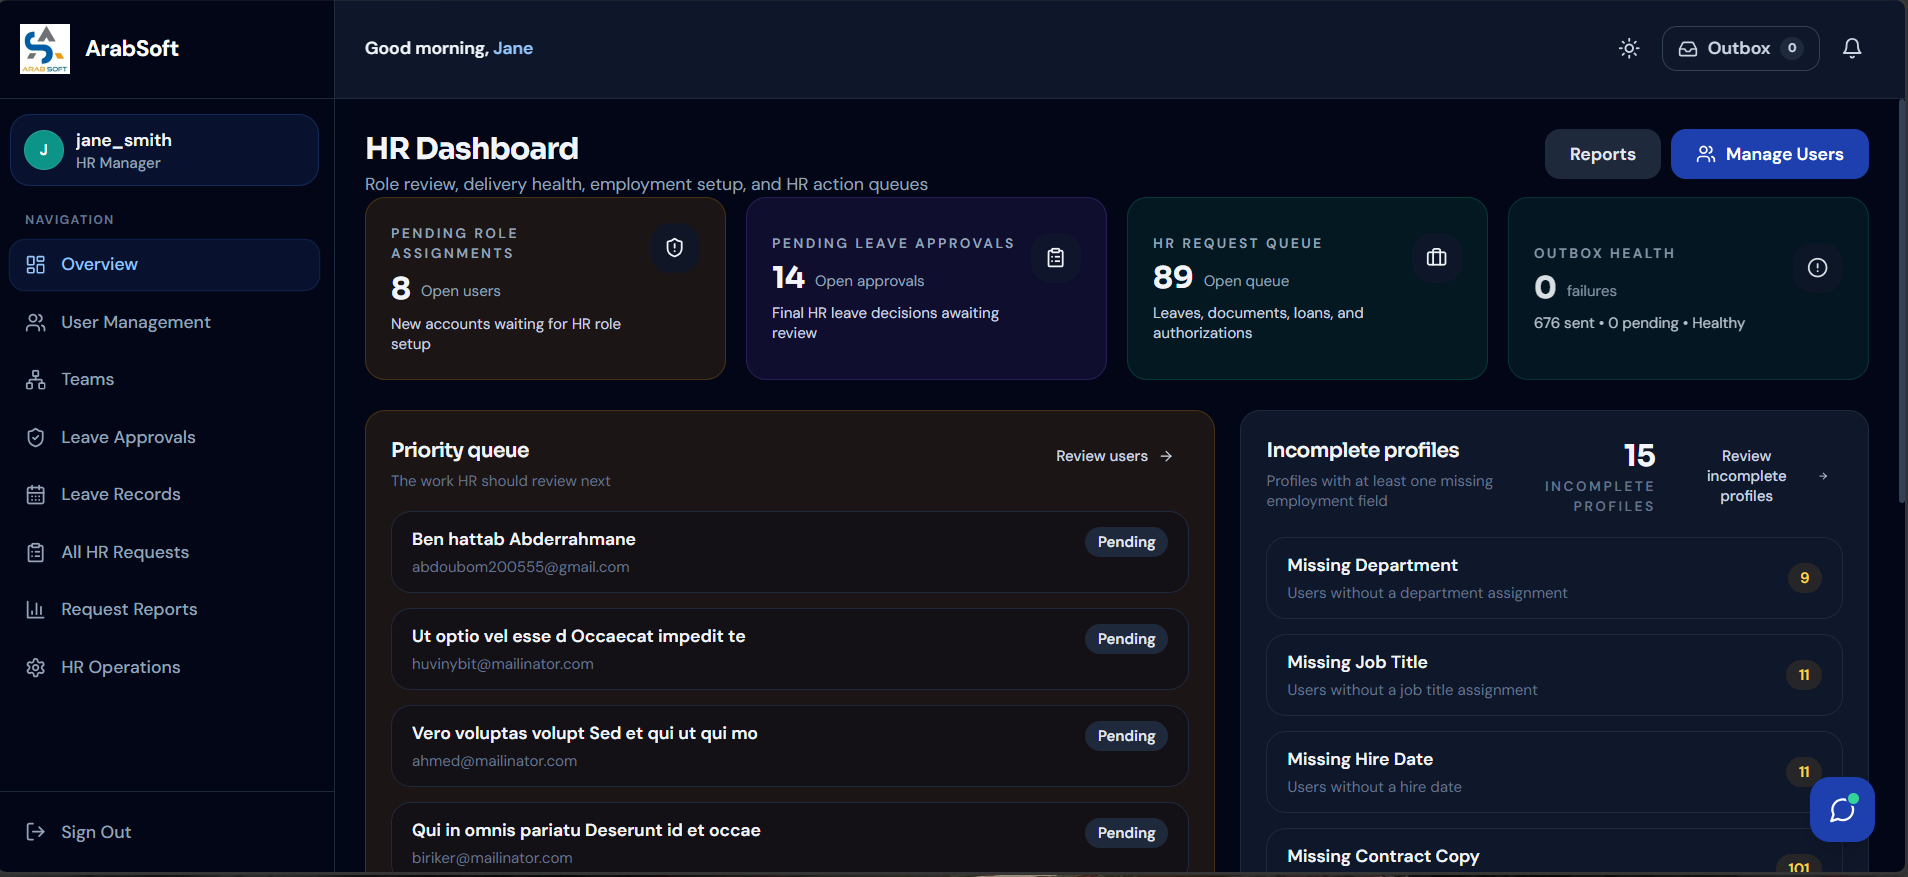
\includegraphics[width=0.95\textwidth,keepaspectratio]{sections/chapitre4/img/sprint4_hr_management_calendar/09_ui_screenshots/sprint4_hr_dashboard.png}
  \caption{HR Dashboard Interface}
  \label{fig:sprint4_hr_dashboard_ui}
\end{figure}

\Needspace{7.2cm}
\begin{figure}[H]
  \centering
  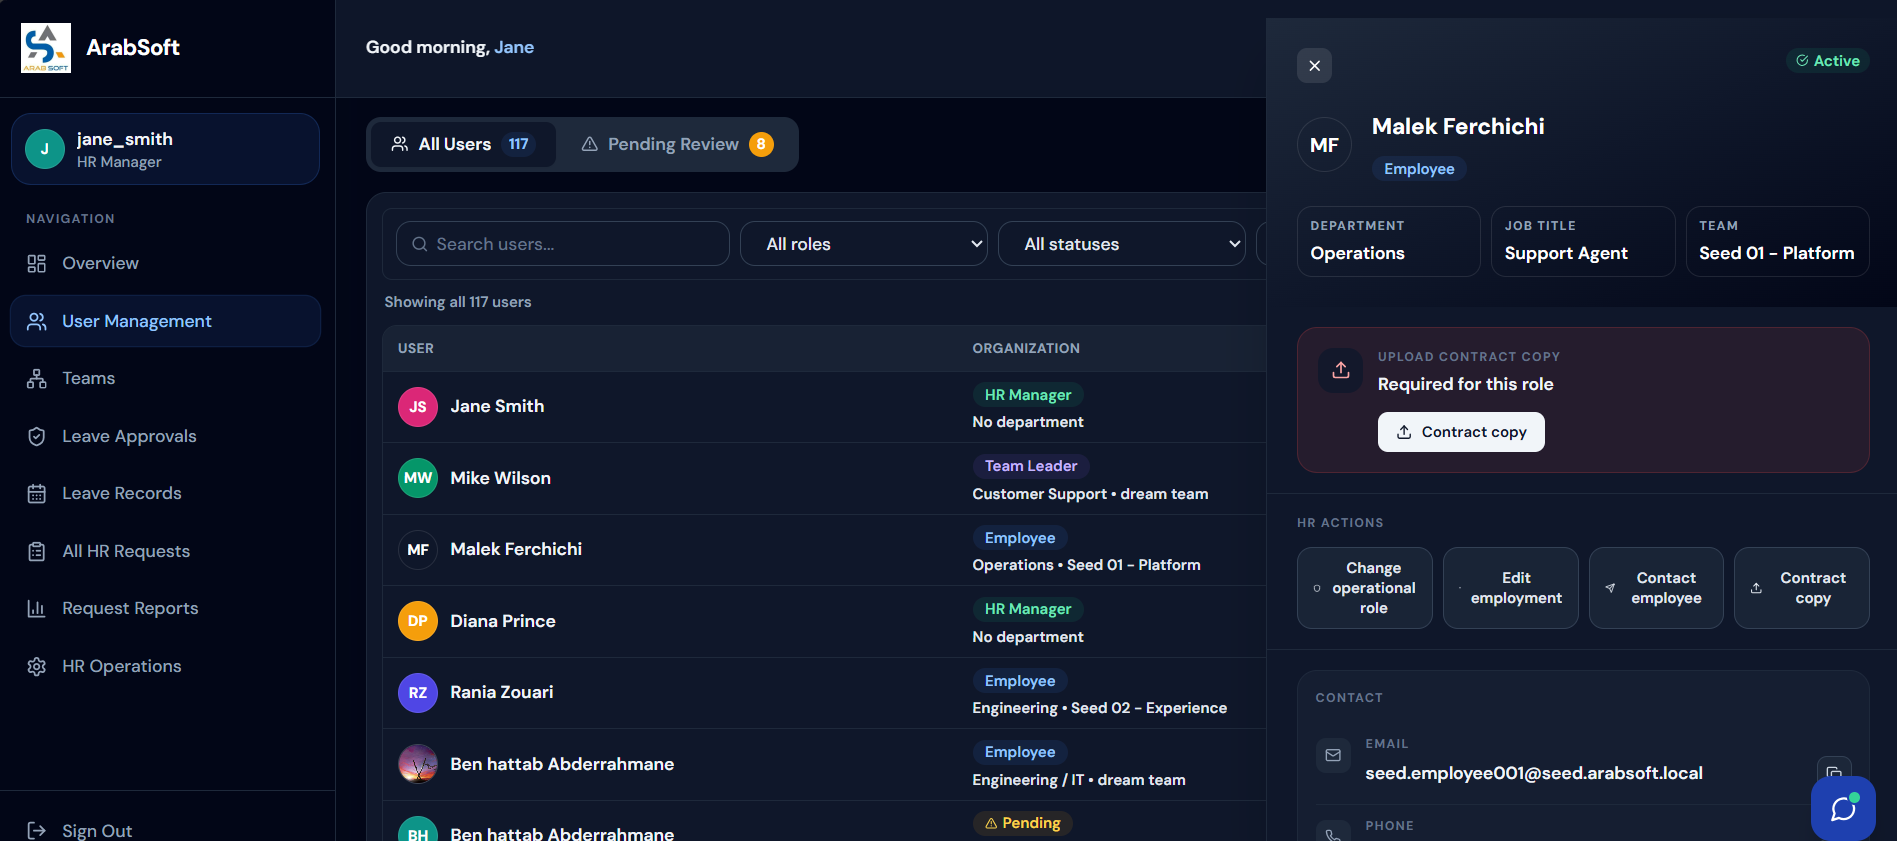
\includegraphics[width=0.95\textwidth,keepaspectratio]{sections/chapitre4/img/sprint4_hr_management_calendar/09_ui_screenshots/sprint4_hr_user_management.png}
  \caption{HR User Management Interface}
  \label{fig:sprint4_hr_user_management_ui}
\end{figure}

\Needspace{7.2cm}
\begin{figure}[H]
  \centering
  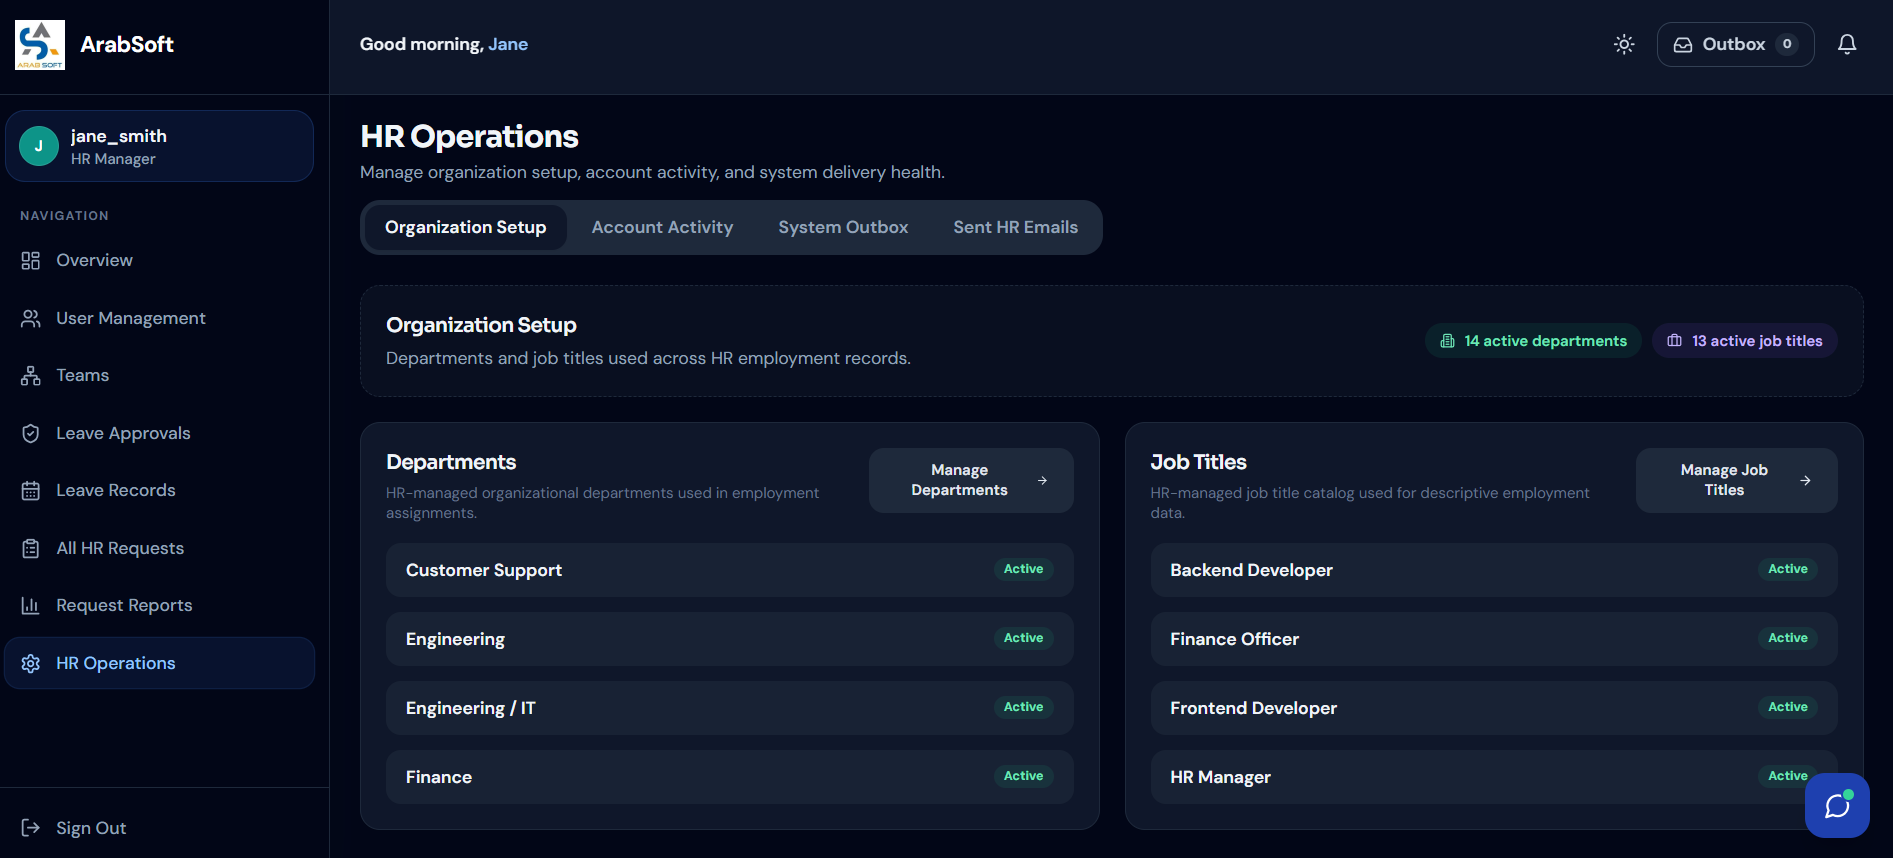
\includegraphics[width=0.95\textwidth,keepaspectratio]{sections/chapitre4/img/sprint4_hr_management_calendar/09_ui_screenshots/sprint4_organization_reference_data.png}
  \caption{Team Management Interface}
  \label{fig:sprint4_team_management_ui}
\end{figure}

\Needspace{7.2cm}
\begin{figure}[H]
  \centering
  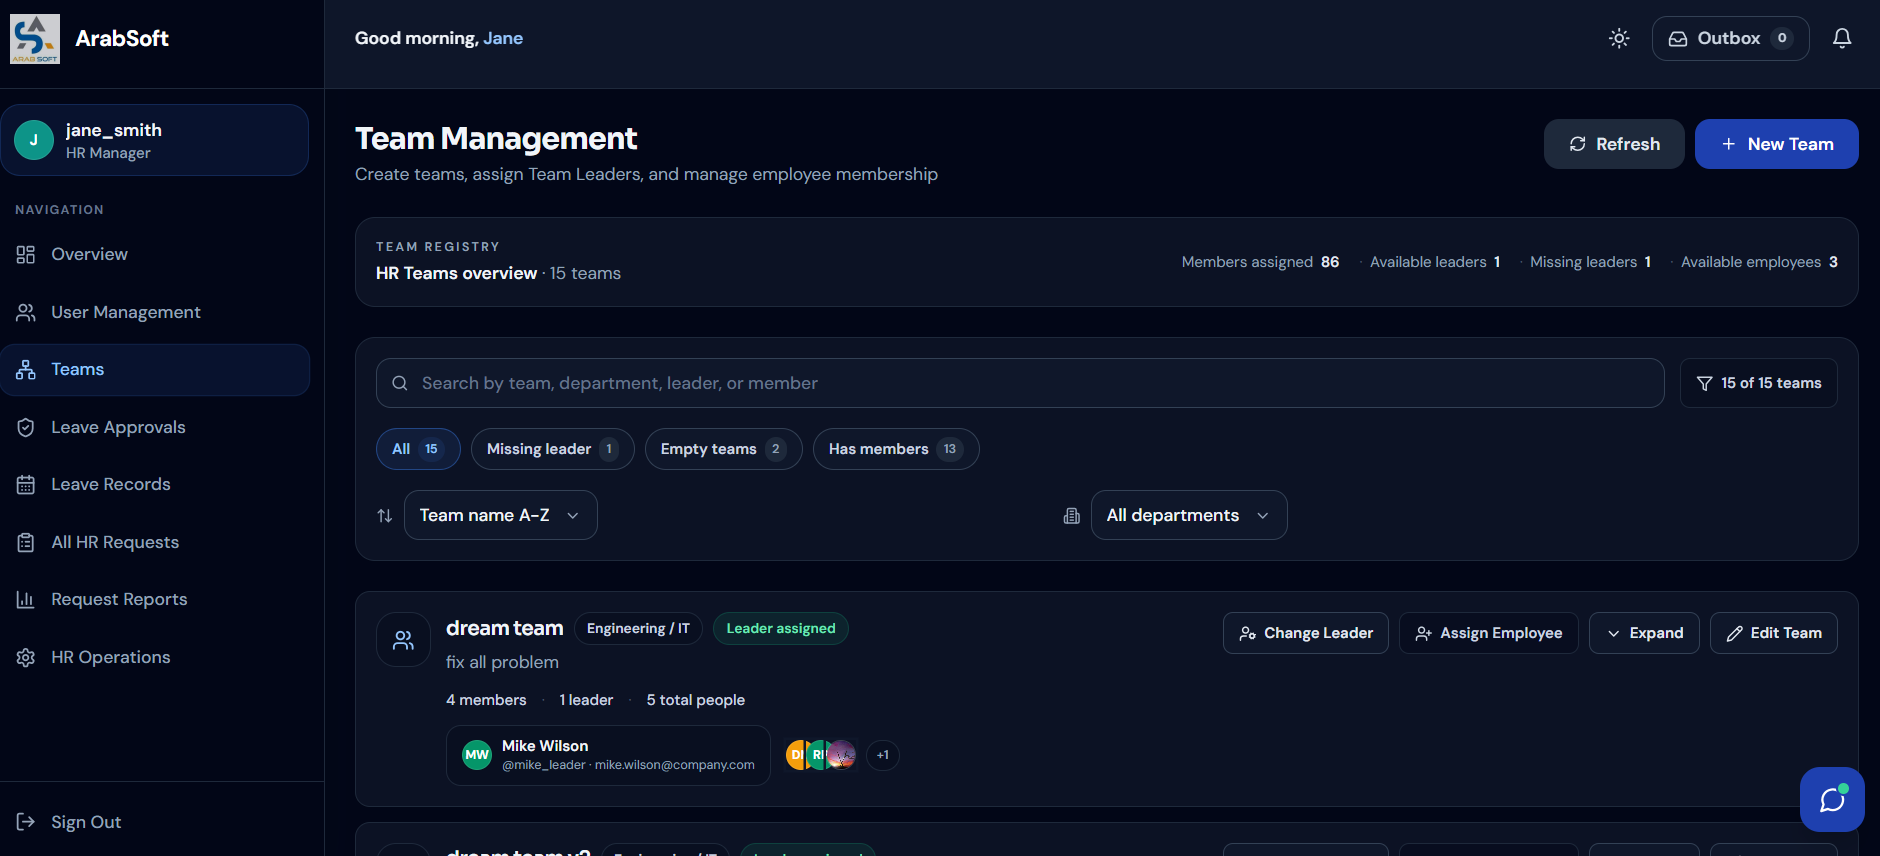
\includegraphics[width=0.95\textwidth,keepaspectratio]{sections/chapitre4/img/sprint4_hr_management_calendar/09_ui_screenshots/sprint4_team_management.png}
  \caption{Organization Reference Data Interface}
  \label{fig:sprint4_organization_reference_data_ui}
\end{figure}

\Needspace{12cm}
\begin{figure}[H]
  \centering
  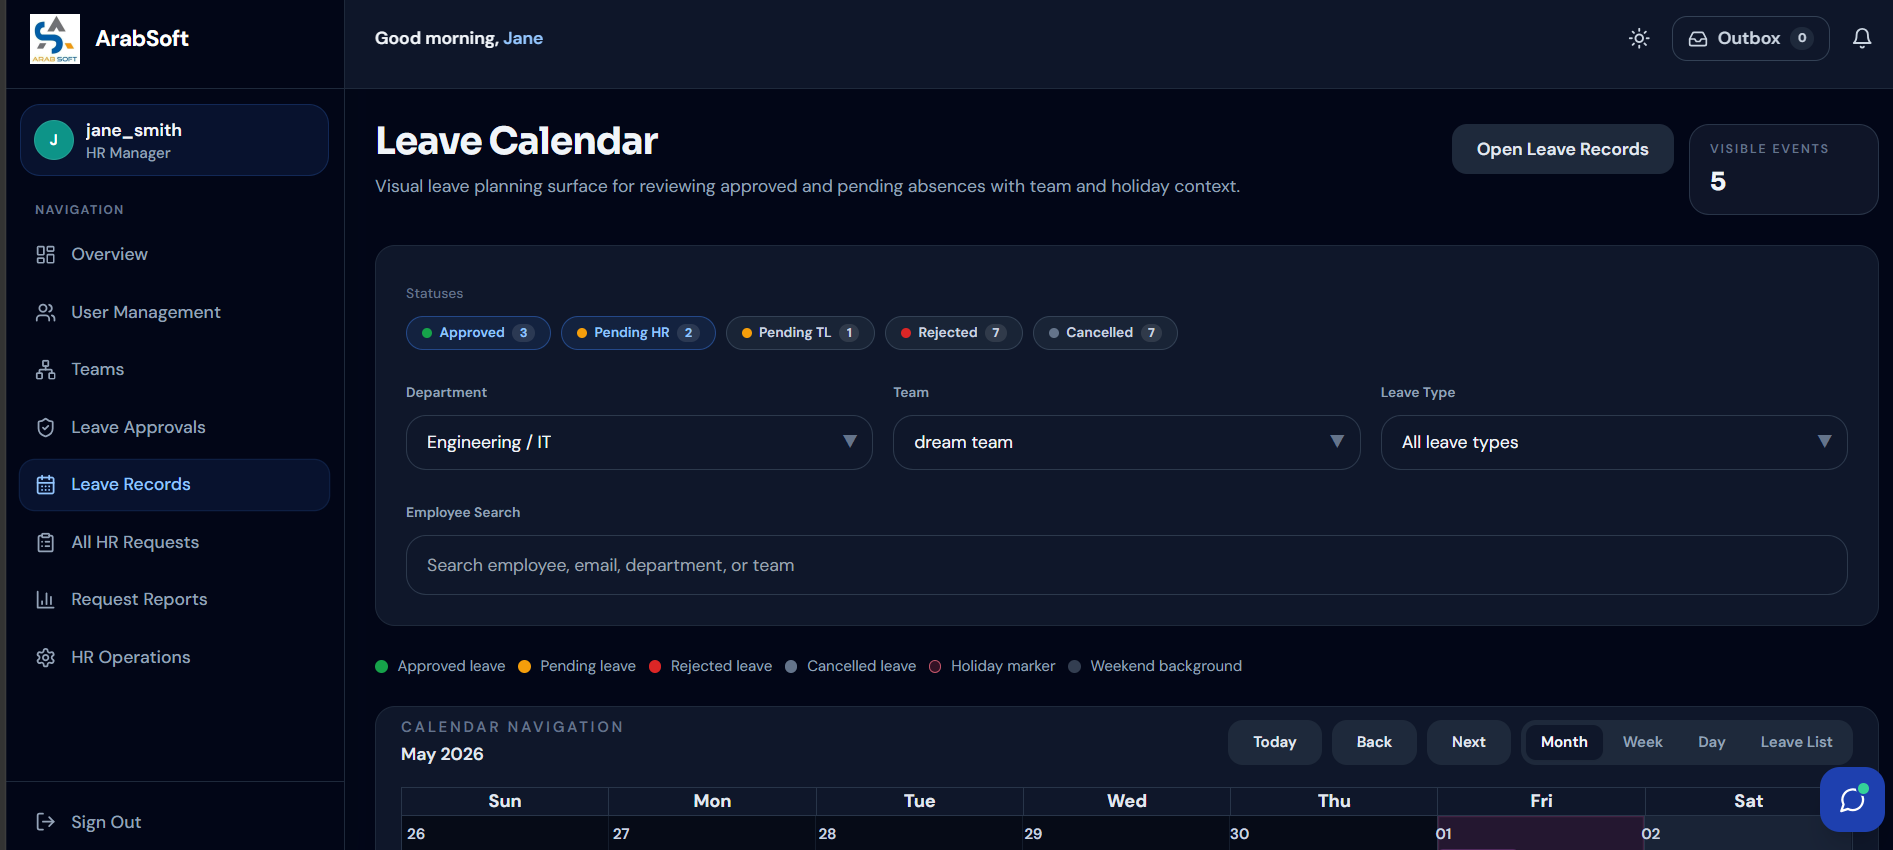
\includegraphics[width=0.95\textwidth,keepaspectratio]{sections/chapitre4/img/sprint4_hr_management_calendar/09_ui_screenshots/sprint4_hr_leave_calendar1.png}
  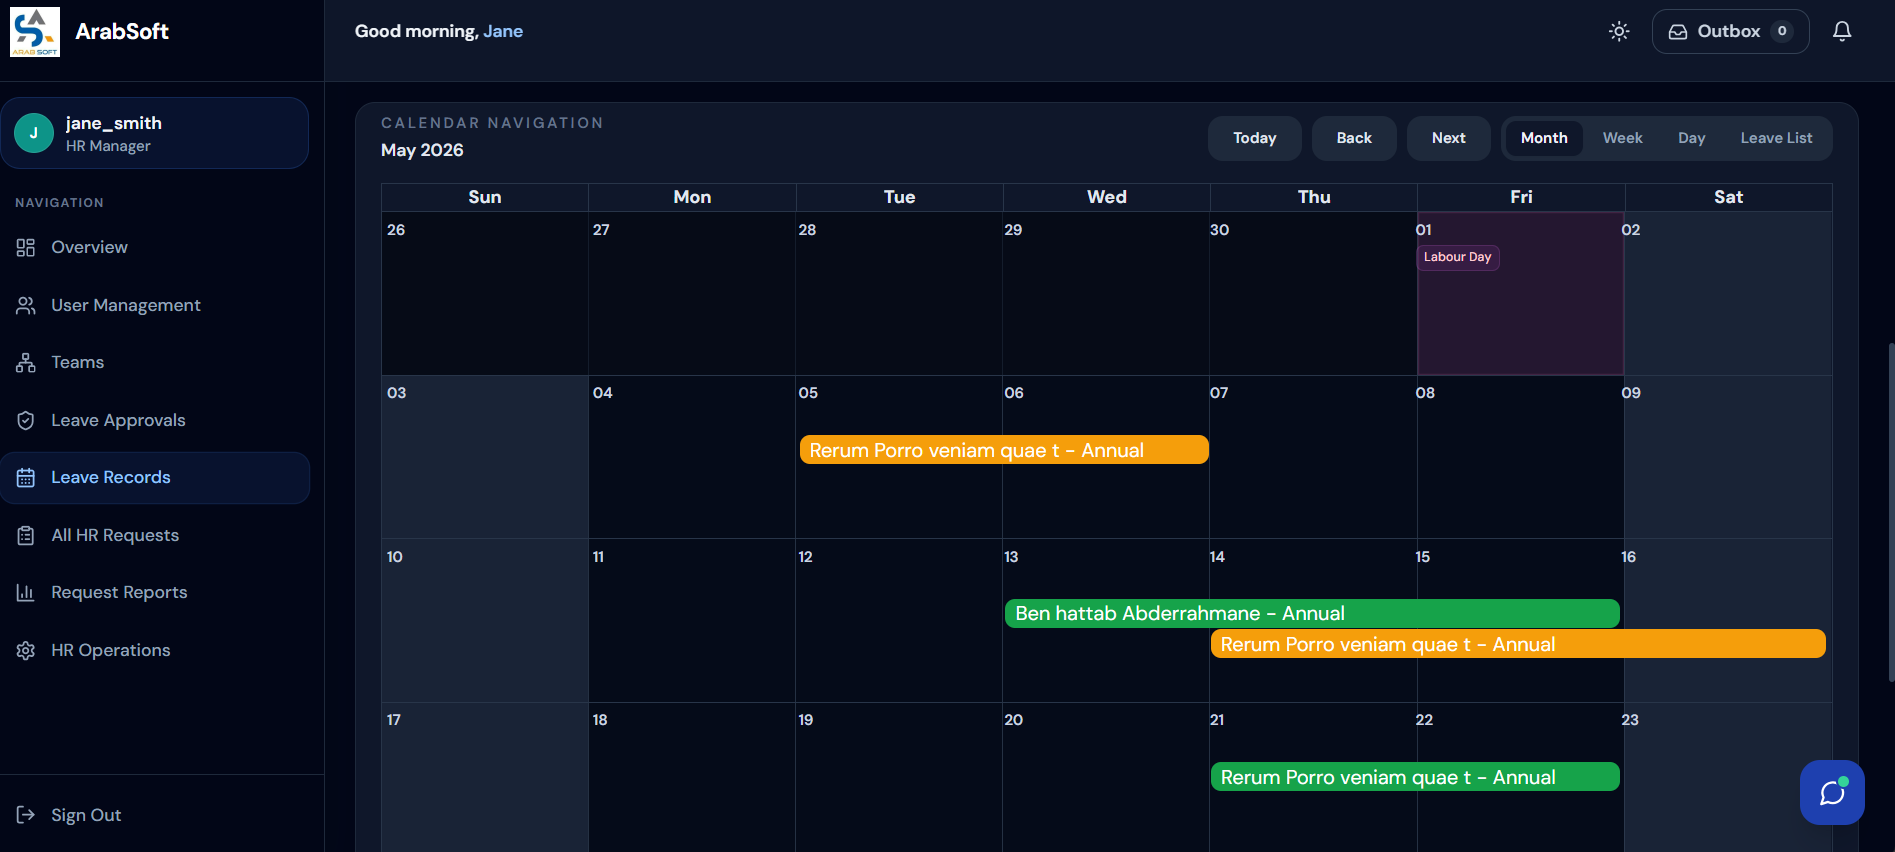
\includegraphics[width=0.95\textwidth,keepaspectratio]{sections/chapitre4/img/sprint4_hr_management_calendar/09_ui_screenshots/sprint4_hr_leave_calendar2.png}
  \caption{HR Leave Calendar Interface}
  \label{fig:sprint4_hr_leave_calendar_ui}
\end{figure}

\ReportSubsection{III.5 Sprint Review}{\hspace{0.5cm} 5. Sprint Review}

{\fontsize{12}{18}\selectfont
\setlength{\parindent}{1.2cm}
\setlength{\parskip}{6pt}

\indent Sprint 4 covered HR management and calendar supervision. The sprint included HR user management, employee records, role assignment, account activation and deactivation, department and job title management, team creation, team leader assignment, team membership changes, and leave calendar consultation. Team leaders also received a dedicated team calendar and leave-decision support within their team scope.

}

\ReportSubsection{III.6 Sprint Retrospective}{\hspace{0.5cm} 6. Sprint Retrospective}

{\fontsize{12}{18}\selectfont
\setlength{\parindent}{1.2cm}
\setlength{\parskip}{6pt}

\begin{table}[H]
\centering
\renewcommand{\arraystretch}{1.5}
\setlength{\tabcolsep}{6pt}
\begin{tabular}{|>{\centering\bfseries\arraybackslash}m{5.2cm}|>{\centering\bfseries\arraybackslash}m{5.2cm}|}
\hline
\rowcolor{blue!20}
\textbf{What went well} & \textbf{What needs improvement} \\
\hline
Sprint 4 features were completed and integrated successfully.
&
Some code still needs final cleanup and consistency checks.
\\
\hline
HR user, team, and calendar workflows now work in the platform.
&
A few screens need small frontend adjustments after final testing.
\\
\hline
\end{tabular}
\caption{Sprint Retrospective -- Sprint 4}
\label{tab:sprint4_retrospective}
\end{table}

}

\clearpage
% ============================================================
%  CONCLUSION
% ============================================================
\ReportSection{Conclusion}{Conclusion}

{\fontsize{12}{18}\selectfont
\setlength{\parindent}{1.2cm}
\setlength{\parskip}{6pt}

\indent This chapter presented Release 2 of the ArabSoft platform. Sprint 3 introduced the administrative request workflows for documents, loans, and authorizations, including HR decisions, request history, notifications, meetings, and final-file handling. Sprint 4 extended the platform with HR management and calendar supervision by covering user records, roles, account status, organization reference data, teams, team membership, and role-aware leave calendar views.

\indent Together, these two sprints added request workflows, HR supervision, team management, and leave calendar access to the platform. The next release covers project tracking, task management, report export, and AI-assisted support features.

}
